% \newpage
\subsection{Introduction}
Nowadays, web applications are dominating online systems.
From Google to Facebook and others, web applications are widely deployed across organizations and continuously accessed by end-users, both for their personal and professional daily tasks.
In practice, the development of these web applications heavily relies on a wide ecosystem of \emph{web frameworks}, which are intended to ease and foster the development process.
However, once deployed, the applications developed with such web frameworks do not exhibit the same performances, as reported by the \emph{Web Framework Benchmarks} periodically published by the \textsc{TechEmpower} company.\footnote{\url{https://www.techempower.com/benchmarks}}
Thanks to such benchmarks, developers can take informed decisions on the most efficient technology to adopt to implement their web applications.
Unfortunately, one can regret that developers and benchmark providers mostly focus on popularity and performance criteria when picking a web framework, with fewer considerations for the resource consumption implications of their choice.
This is all the more regrettable that cloud providers are more and more adopted by developers to host these web applications.
While cloud providers offer a convenient elastic provision of resources to scale according to application requirements, this convenience may induce critical costs for their business.
% , their pricing model focuses on this resource consumption by charging the application owner.

Beyond the economical cost of web applications, one can also question the global impact of web applications on worldwide carbon emissions.
Given the tremendous success of web applications, their deployment has severely increased over the last years, thus causing a rebound effect on the power consumption of server infrastructure---being hosted or supported by cloud providers.
While one can challenge the relevance of features that are continuously deployed by developers to keep engaging end-users, reconciling economical and environmental concerns remains an open challenge to address.

Given this context, this section intends to address this challenge by investigating the energy footprint of web frameworks.
In particular, we aim to support the developers of web applications with relevant guidelines that can help them to choose the web framework that is not only the most popular or provides the best performance but also exhibits a low energy footprint.
By minimizing the energy consumed to process user requests, with no service quality penalty, developers can reduce the operational cost of their web applications and contribute to reducing worldwide carbon emissions of ICT.
% While we assume this choice does not conflict with the appropriate selection of relevant user features, this topic remains out of the scope of this paper.

To achieve this objective, we leverage the \textsc{TechEmpower} \emph{Web Framework Benchmarks} to incorporate server-side energy measurements obtained from a software-defined power meter, named \textsc{PowerAPI}~\cite{fieni2020smartwatts}.
These measurements are then analyzed in depth to understand the key criteria that can impact the power consumption of web frameworks and derive guidelines to can support developers to pick the most energy-efficient web frameworks according to their requirements.

% The remainder of this section is organized as follows.
\subsubsection{Comparison of Web Frameworks}
Many studies have been conducted to compare the performance of web frameworks.
One can cite \cite{gajewski_analysis_2019} who compared two of the most famous Java frameworks---Play and Spring---or the work of \cite{benmoussa_new_2019} who compared different PHP frameworks using 6 criteria: intrinsic durability, industrialized solution, technical adaptability, strategy, technical architecture, and speed.
% TODO : ASK romain if we should remove this  part since it is soa 
% In the previous section, we observed that all those 6 criteria have their own wait when it comes to choose which framework to take for a project.
In our context, we push a $7^{th}$ criterion that impacts the economic outcome of the project.

\subsubsection{Energy Efficiency in Software Engineering}
In their paper~\cite{pereira_energy_2017}, the authors studied the impact of programming languages on energy, time, and memory by using the CLBG benchmark, where they executed 10 different benchmarks\footnote{\url{https://salsa.debian.org/benchmarksgame-team/benchmarksgame}} across 27 wellknown programming languages~\cite{noauthor_pypl_2018}.
The work of these authors was an extension of a research initiated by the work of \citeauthor{couto2017towards}~\cite{couto2017towards} to measure the impact of programming languages choice in real-life applications, instead of micro-benchmarks.

Irene~\emph{et~al.}~\cite{manotas_investigating_2013} investigated the impact of web servers on energy when handling web applications.
They analyzed 7 applications executed within 4 servers in 38 different scenarios.
The authors showed that the energy greatly depends on the web server, but the impact of the application may also influence the energy behavior of the server.
In their approach, they used measured the energy consumption during the integration tests, while we are interested in simulating more realistic workloads, and isolating the energy consumption of the server from the client's one.

%notes 
% instead of focusing on energy or execution time we change the paradigm into efficiency and average power 
Other works have been achieved on measuring the energy consumption of the client applications, as an example \cite{philippot_characterization_2014} concluded that there is a variation among the different websites and the impact of the browser on this energy consumption.

\subsection{Research questions \note{missing}}


\newcommand\duration{20}
\newcommand\parallelclient{512}
\subsection{Experimental Protocol}
In this section, we describe the environment we used during the experiments, covering hardware features, experiments of the framework and the methodology.

\subsubsection{Measurement Context}
The purpose of this experiment is to highlight the energy impact of the technology stack used to develop a web application once in production.

\paragraph{Candidate Frameworks}
Overall, we selected 210 web frameworks to be evaluated in this study.
Each framework may have multiple configurations, based on the database, alternative interpreters, etc.
Table~\ref{tab:frameworks_all} lists the frameworks that we selected for this study.

% 

% \begin{longtable}{lll}
%     \toprule
%     framework        & language    & alternative implementations                        \\
%     \midrule
%     \endhead
%     \midrule
%     \multicolumn{3}{r}{{Continued on next page}}                                        \\
%     \midrule
%     \endfoot

%     \bottomrule
%     \endlastfoot
%     pico.v           & V           &                                                    \\
%     dylan            & Dylan       &                                                    \\
%     sinatra-sequel   & Ruby        & postgres passenger-mri postgres-passenger-mri...   \\
%     agoo             & Ruby        &                                                    \\
%     rack             & Ruby        & unicorn falcon                                     \\
%     h2o\_mruby       & Ruby        &                                                    \\
%     rails            & Ruby        & postgresql unicorn                                 \\
%     grape            & Ruby        & unicorn                                            \\
%     roda-sequel      & Ruby        & postgres passenger-mri postgres-passenger-mri...   \\
%     rack-sequel      & Ruby        & postgres passenger-mri postgres-passenger-mri...   \\
%     sinatra          & Ruby        & postgres passenger-mri postgres-passenger-mri...   \\
%     padrino          & Ruby        & unicorn                                            \\
%     ninglex          & Common Lisp &                                                    \\
%     ningle           & Common Lisp &                                                    \\
%     woo              & Common Lisp &                                                    \\
%     grails           & Groovy      &                                                    \\
%     hot              & Groovy      & mongodb postgres mysql                             \\
%     plack            & Perl        & async                                              \\
%     kelp             & Perl        & mongodb                                            \\
%     dancer           & Perl        &                                                    \\
%     mojolicious      & Perl        &                                                    \\
%     web-simple       & Perl        &                                                    \\
%     cowboy           & Erlang      &                                                    \\
%     elli             & Erlang      &                                                    \\
%     chicagoboss      & Erlang      &                                                    \\
%     mochiweb         & Erlang      &                                                    \\
%     opium            & OCaml       & haproxy                                            \\
%     morph            & OCaml       & static                                             \\
%     webmachine       & OCaml       & haproxy                                            \\
%     vertx-web-scala  & Scala       &                                                    \\
%     http4s           & Scala       &                                                    \\
%     akka-http        & Scala       & slick-postgres                                     \\
%     fintrospect      & Scala       &                                                    \\
%     finagle          & Scala       &                                                    \\
%     colossus         & Scala       &                                                    \\
%     finatra          & Scala       &                                                    \\
%     blaze            & Scala       &                                                    \\
%     play2-scala      & Scala       & netty anorm anorm-netty reactivemongo reactiv...   \\
%     finch            & Scala       &                                                    \\
%     scalene          & Scala       &                                                    \\
%     cask             & Scala       &                                                    \\
%     youi             & Scala       &                                                    \\
%     httpbeast        & Nim         &                                                    \\
%     prologue         & Nim         &                                                    \\
%     basolato         & Nim         &                                                    \\
%     jester           & Nim         &                                                    \\
%     falco            & F\#         &                                                    \\
%     frank            & F\#         &                                                    \\
%     suave            & F\#         &                                                    \\
%     giraffe          & F\#         & utf8json utf8direct stripped                       \\
%     zebra            & F\#         & simple                                             \\
%     vapor            & Swift       & fluent sql-kit postgres                            \\
%     swift-nio        & Swift       &                                                    \\
%     perfect          & Swift       & mysql postgresql mongodb                           \\
%     kitura           & Swift       & postgres postgres-orm postgres-orm-codable mo...   \\
%     racket           & Racket      &                                                    \\
%     vsgi             & Vala        &                                                    \\
%     valum            & Vala        &                                                    \\
%     wsgi             & Python      &                                                    \\
%     hug              & Python      &                                                    \\
%     crax             & Python      &                                                    \\
%     falcon           & Python      & py3 pypy2                                          \\
%     uvicorn          & Python      &                                                    \\
%     flask            & Python      & raw pypy pypy2 pypy2-raw nginx-uwsgi               \\
%     responder        & Python      &                                                    \\
%     klein            & Python      &                                                    \\
%     blacksheep       & Python      &                                                    \\
%     apidaora         & Python      & core                                               \\
%     bottle           & Python      & pypy2 raw nginx-uwsgi                              \\
%     japronto         & Python      &                                                    \\
%     api\_hour        & Python      & mysql json dbs plaintext                           \\
%     weppy            & Python      & py3 pypy2 nginx-uwsgi                              \\
%     starlette        & Python      &                                                    \\
%     emmett           & Python      &                                                    \\
%     sanic            & Python      &                                                    \\
%     aiohttp          & Python      & pg-raw                                             \\
%     tornado          & Python      & pypy2 postgresql-raw py3 py3-uvloop                \\
%     uwsgi            & Python      & nginx-uwsgi                                        \\
%     pyramid          & Python      & py2                                                \\
%     morepath         & Python      &                                                    \\
%     vibora           & Python      &                                                    \\
%     web2py           & Python      & optimized                                          \\
%     django           & Python      & postgresql                                         \\
%     cherrypy         & Python      & py3                                                \\
%     eve              & Python      &                                                    \\
%     webware          & Python      &                                                    \\
%     spyne            & Python      & raw nginx-uwsgi                                    \\
%     fastapi          & Python      & orjson                                             \\
%     quart            & Python      & uvicorn                                            \\
%     turbogears       & Python      &                                                    \\
%     m-web-server     & mumps       &                                                    \\
%     urweb            & Ur          & mysql cache mysql-cache                            \\
%     rouille          & Rust        &                                                    \\
%     warp-rust        & Rust        &                                                    \\
%     thruster         & Rust        &                                                    \\
%     ntex             & Rust        & db raw                                             \\
%     iron             & Rust        &                                                    \\
%     actix            & Rust        & core raw diesel pg                                 \\
%     roa              & Rust        & core tokio diesel pg sqlx                          \\
%     saphir           & Rust        &                                                    \\
%     may-minihttp     & Rust        &                                                    \\
%     rocket           & Rust        &                                                    \\
%     tokio-minihttp   & Rust        &                                                    \\
%     nickel           & Rust        &                                                    \\
%     hyper            & Rust        & db                                                 \\
%     gotham           & Rust        &                                                    \\
%     kooby            & Kotlin      &                                                    \\
%     pronghorn        & Kotlin      &                                                    \\
%     http4k           & Kotlin      & apache apache4 jetty ktorcio ktornetty netty ...   \\
%     ktor             & Kotlin      & jetty cio jasync reactivepg                        \\
%     hexagon          & Kotlin      & resin-mongodb jetty-postgresql resin-postgresql    \\
%     elixir-plug-ecto & Elixir      &                                                    \\
%     phoenix          & Elixir      &                                                    \\
%     fiber            & Go          & prefork                                            \\
%     webgo            & Go          &                                                    \\
%     gnet             & Go          &                                                    \\
%     goframe          & Go          &                                                    \\
%     revel            & Go          & fast raw jet qbs                                   \\
%     echo             & Go          &                                                    \\
%     gramework        & Go          &                                                    \\
%     gin              & Go          & scratch                                            \\
%     atreugo          & Go          & prefork                                            \\
%     beego            & Go          & orm-mysql                                          \\
%     kami             & Go          &                                                    \\
%     falcore          & Go          &                                                    \\
%     goji             & Go          &                                                    \\
%     clevergo         & Go          &                                                    \\
%     fasthttp         & Go          & prefork                                            \\
%     aah              & Go          & mysql postgresql                                   \\
%     gearbox          & Go          & prefork                                            \\
%     martini          & Go          &                                                    \\
%     go               & Go          & pgx pgx-easyjson pgx-quicktemplate pgx-prefor...   \\
%     evio             & Go          & stdlib                                             \\
%     chi              & Go          & scratch prefork gojay gojay-prefork sjson sjs...   \\
%     warp             & Haskell     & hasql mysql-haskell                                \\
%     yesod            & Haskell     & mongodb-raw                                        \\
%     wizzardo-inline  & Haskell     &                                                    \\
%     snap             & Haskell     &                                                    \\
%     spock            & Haskell     &                                                    \\
%     ihp              & Haskell     &                                                    \\
%     servant          & Haskell     & beam psql-simple                                   \\
%     stream           & Dart        &                                                    \\
%     start            & Dart        &                                                    \\
%     angel            & Dart        & postgres                                           \\
%     redstone         & Dart        & mongodb                                            \\
%     dart             & Dart        &                                                    \\
%     aqueduct         & Dart        &                                                    \\
%     aspcore-vb-mw    & VB          & ado-pg ado-my                                      \\
%     spider-gazelle   & Crystal     &                                                    \\
%     toro             & Crystal     &                                                    \\
%     onyx             & Crystal     &                                                    \\
%     h2o.cr           & Crystal     &                                                    \\
%     kemal            & Crystal     & concurrent-queries                                 \\
%     lucky            & Crystal     &                                                    \\
%     crystal          & Crystal     & radix                                              \\
%     grip             & Crystal     &                                                    \\
%     orion            & Crystal     &                                                    \\
%     amber            & Crystal     &                                                    \\
%     raze             & Crystal     &                                                    \\
%     collie           & D           & ldc                                                \\
%     vibed            & D           & dmd-pgsql ldc ldc-pgsql                            \\
%     hunt             & D           &                                                    \\
%     macchiato        & Clojure     &                                                    \\
%     aleph            & Clojure     &                                                    \\
%     luminus          & Clojure     &                                                    \\
%     pedestal         & Clojure     &                                                    \\
%     compojure        & Clojure     & raw                                                \\
%     http-kit         & Clojure     & raw                                                \\
%     duct             & Clojure     & mongodb httpkit aleph immutant                     \\
%     reitit           & Clojure     & jdbc async                                         \\
%     nestjs           & TypeScript  & mysql mongo fastify fastify-mysql fastify-mongo    \\
%     typescript-rest  & TypeScript  &                                                    \\
%     deno             & TypeScript  &                                                    \\
%     dropwizard       & Java        & mongodb postgres jdbi-postgres                     \\
%     httpserver       & Java        & postgres                                           \\
%     quarkus          & Java        & pgclient                                           \\
%     jooby            & Java        & netty jaxrs jetty pgclient                         \\
%     undertow         & Java        & postgresql                                         \\
%     tapestry         & Java        &                                                    \\
%     vertx-web        & Java        & mongodb postgres susom-postgres                    \\
%     jlhttp           & Java        & postgres                                           \\
%     voovan           & Java        &                                                    \\
%     play2-java       & Java        & netty ebean-hikaricp ebean-hikaricp-netty jpa...   \\
%     officefloor      & Java        & raw tpr micro thread\_affinity netty spring\_data  \\
%     jersey           & Java        &                                                    \\
%     proteus          & Java        & mysql                                              \\
%     light-4j         & Java        &                                                    \\
%     activeweb        & Java        & jackson                                            \\
%     minijax          & Java        &                                                    \\
%     jetty            & Java        & servlet                                            \\
%     spark            & Java        &                                                    \\
%     grizzly          & Java        & jersey                                             \\
%     servlet          & Java        & lib-native mysql postgresql                        \\
%     tio-mvc          & Java        &                                                    \\
%     baratine         & Java        &                                                    \\
%     servicetalk      & Java        &                                                    \\
%     play1            & Java        &                                                    \\
%     ninja-standalone & Java        &                                                    \\
%     nanohttpd        & Java        &                                                    \\
%     simple-server    & Java        &                                                    \\
%     restexpress      & Java        & mysql-raw                                          \\
%     javalin          & Java        &                                                    \\
%     jawn             & Java        &                                                    \\
%     redkale          & Java        & postgres                                           \\
%     revenj-jvm       & Java        &                                                    \\
%     spring-webflux   & Java        & mongo pgclient rxjdbc jdbc                         \\
%     firenio          & Java        & http-lite                                          \\
%     curacao          & Java        &                                                    \\
%     bayou            & Java        &                                                    \\
%     wizzardo-http    & Java        &                                                    \\
%     netty            & Java        &                                                    \\
%     armeria          & Java        &                                                    \\
%     vertx            & Java        & postgres                                           \\
%     comsat           & Java        & servlet-undertow webactors-netty webactors-un...   \\
%     ratpack          & Java        & jdbc pgclient                                      \\
%     wicket           & Java        &                                                    \\
%     wildfly-ee       & Java        &                                                    \\
%     undertow-jersey  & Java        & hikaricp                                           \\
%     micronaut        & Java        &                                                    \\
%     servlet3         & Java        & sync                                               \\
%     act              & Java        & hibernate-pgsql hibernate-pgsql-rythm hiberna...   \\
%     blade            & Java        &                                                    \\
%     rapidoid         & Java        & mysql postgres http-fast                           \\
%     smart-socket     & Java        &                                                    \\
%     gemini           & Java        & mysql postgres                                     \\
%     greenlightning   & Java        &                                                    \\
%     helidon          & Java        &                                                    \\
%     spring           & Java        & jpa mongo                                          \\
%     codeigniter      & PHP         &                                                    \\
%     fat-free         & PHP         & raw                                                \\
%     php              & PHP         & activerecord raw7-tcp pgsql-raw h2o unit pool...   \\
%     cakephp          & PHP         &                                                    \\
%     ubiquity         & PHP         & workerman swoole swoole-mysql roadrunner road...   \\
%     fuel             & PHP         &                                                    \\
%     sw-fw-less       & PHP         &                                                    \\
%     hyperf           & PHP         & raw micro                                          \\
%     kumbiaphp        & PHP         & raw workerman workerman-mysql                      \\
%     workerman        & PHP         & pgsql async                                        \\
%     lumen            & PHP         & swoole                                             \\
%     peachpie         & PHP         &                                                    \\
%     yii2             & PHP         & raw                                                \\
%     php-ngx          & PHP         & mysql pgsql async                                  \\
%     laravel          & PHP         & swoole                                             \\
%     symfony          & PHP         & raw swoole                                         \\
%     imi              & PHP         & query-builder raw                                  \\
%     webman           & PHP         &                                                    \\
%     phalcon          & PHP         & mongodb micro                                      \\
%     slim             & PHP         &                                                    \\
%     amp              & PHP         &                                                    \\
%     hhvm             & PHP         &                                                    \\
%     spiral           & PHP         &                                                    \\
%     swoole           & PHP         & postgres no-async                                  \\
%     hamlet           & PHP         & swoole workerman                                   \\
%     simps            & PHP         & micro                                              \\
%     one              & PHP         &                                                    \\
%     zend             & PHP         &                                                    \\
%     phpixie          & PHP         &                                                    \\
%     comet            & PHP         & mysql                                              \\
%     nginx            & C           &                                                    \\
%     onion            & C           &                                                    \\
%     duda             & C           &                                                    \\
%     libreactor       & C           & server                                             \\
%     lwan             & C           & lua                                                \\
%     h2o              & C           &                                                    \\
%     facil\_io        & C           &                                                    \\
%     octane           & C           &                                                    \\
%     polkadot         & JavaScript  & mysql postgres mongodb                             \\
%     restify          & JavaScript  &                                                    \\
%     hapi             & JavaScript  & nginx mysql postgres                               \\
%     nodejs           & JavaScript  & chakra mongodb mongodb-raw mysql postgres          \\
%     restana          & JavaScript  &                                                    \\
%     es4x             & JavaScript  &                                                    \\
%     sailsjs          & JavaScript  & postgres                                           \\
%     just             & JavaScript  &                                                    \\
%     fastify          & JavaScript  & mysql postgres                                     \\
%     ringojs          & JavaScript  & convenient                                         \\
%     express          & JavaScript  & chakra mongodb mysql postgres graphql-mysql g...   \\
%     koa              & JavaScript  & mysql postgres                                     \\
%     0http            & JavaScript  &                                                    \\
%     openresty        & Lua         &                                                    \\
%     octopus          & Lua         &                                                    \\
%     lapis            & Lua         &                                                    \\
%     easyrpc          & C\#         &                                                    \\
%     aspcore-mono     & C\#         & pg mw mw-pg mw-my mvc mvc-pg mvc-my                \\
%     servicestack     & C\#         &                                                    \\
%     tetsuweb         & C\#         &                                                    \\
%     beetlex          & C\#         & core core-updb debug                               \\
%     aspcore          & C\#         & pgo ado-pg ado-pg-up pgo-pg pgo-pg-up mw mw-j...   \\
%     revenj           & C\#         &                                                    \\
%     carter           & C\#         &                                                    \\
%     aspnet-mono-ngx  & C\#         & jn ss my my-ef                                     \\
%     genhttp          & C\#         &                                                    \\
%     ben              & C\#         & pg                                                 \\
%     evhttp-sharp     & C\#         &                                                    \\
%     zysocket-v       & C\#         &                                                    \\
%     nancy            & C\#         & netcore                                            \\
%     aspcore-corert   & C\#         &                                                    \\
%     cuehttp          & C++         &                                                    \\
%     libhttpserver    & C++         &                                                    \\
%     ffead-cpp        & C++         & mongo-raw lithium cinatra drogon libreactor h...   \\
%     lithium          & C++         & postgres postgres-batch                            \\
%     wt               & C++         & postgres                                           \\
%     treefrog         & C++         & postgres mongodb                                   \\
%     ulib             & C++         & plaintext\_fit json json\_fit mysql postgres po... \\
%     cppcms           & C++         & postgres                                           \\
%     oatpp            & C++         & no-mp async async-no-mp                            \\
%     poco             & C++         &                                                    \\
%     silicon          & C++         &                                                    \\
%     cutelyst         & C++         & pf-apg pf-pg pf-my thread thread-apg thread-p...   \\
%     drogon           & C++         & core                                               \\
%     cinatra          & C++         &                                                    \\
%     libsniper        & C++         &                                                    \\
%     cpoll\_cppsp     & C++         & raw postgres-raw postgres-raw-threadpool           \\
% \end{longtable}


Table~\ref{table:frameworks_count} highlights the number of frameworks used in the experiment per category of benchmark.
As we see in this table, some of the frameworks worked on certain conditions, while they failed on other benchmarks, such as Nickel (based on Rust).
While it might be one of the most energy-efficient Rust frameworks, Nickel does not work with databases.
Therefore, it cannot be used for any situation, but if a (stateless) web application does not interact with a database, then it might be the best choice.
Many reasons are behind the observed failures, either there was no implementation or some errors were raised when handling the request.

\paragraph{Remark}
We decided to skip the idle part in the validation benchmark since it is not relevant.

\begin{table*}
    \raggedright
    \caption{the number of framework passed per test }
    \label{table:frameworks_count}
    \begin{tabular}{l|c|c|c|c|c|c|c}
        \toprule
        Language    & Bb  & Query & Update & Plaintext & Fortune & Json & Total \\
        \midrule
        c           & 1   & 1     & 1      & 6         & 1       & 5    & 15    \\
        c\#         & 21  & 20    & 14     & 12        & 14      & 17   & 98    \\
        c++         & 27  & 16    & 14     & 20        & 13      & 25   & 115   \\
        cfml        & 2   & 1     & 1      & 1         & 1       & 2    & 8     \\
        clojure     & 8   & 8     & 5      & 6         & 7       & 8    & 42    \\
        common lisp & 2   & /     & /      & /         & /       & 2    & 4     \\
        crystal     & 3   & 1     & /      & 2         & /       & 2    & 8     \\
        d           & 3   & 2     & 1      & 2         & 1       & 3    & 12    \\
        dart        & /   & /     & /      & 2         & /       & 2    & 4     \\
        elixir      & 1   & 1     & /      & /         & /       & 1    & 3     \\
        erlang      & 3   & 2     & /      & 3         & 1       & 3    & 12    \\
        f\#         & /   & /     & /      & 4         & 2       & 8    & 14    \\
        go          & 19  & 18    & 16     & 15        & 15      & 19   & 102   \\
        groovy      & 1   & /     & /      & 1         & /       & 2    & 4     \\
        haskell     & 1   & 1     & 1      & 2         & 1       & 2    & 8     \\
        java        & 20  & 20    & 18     & 26        & 21      & 26   & 131   \\
        javascript  & 19  & 19    & 16     & 14        & 17      & 14   & 99    \\
        julia       & /   & /     & /      & 1         & /       & 1    & 2     \\
        kotlin      & 10  & 9     & 6      & 5         & 5       & 10   & 45    \\
        lua         & 1   & 1     & /      & 1         & 1       & 2    & 6     \\
        nim         & /   & /     & /      & 2         & /       & 3    & 5     \\
        ocaml       & 4   & 4     & 3      & 1         & 2       & 5    & 19    \\
        perl        & 2   & /     & /      & 1         & /       & 2    & 5     \\
        php         & 22  & 18    & 15     & 10        & 12      & 14   & 91    \\
        prolog      & /   & /     & /      & 1         & /       & 1    & 2     \\
        python      & 31  & 21    & 15     & 17        & 16      & 30   & 130   \\
        racket      & 1   & /     & /      & /         & /       & /    & 1     \\
        ruby        & 23  & 15    & 11     & 8         & 12      & 19   & 88    \\
        rust        & 8   & 7     & 6      & 9         & 8       & 10   & 48    \\
        scala       & 7   & 6     & 3      & 8         & 5       & 11   & 40    \\
        swift       & 2   & 2     & /      & 2         & /       & 2    & 8     \\
        typescript  & 4   & 2     & 2      & 3         & 2       & 6    & 19    \\
        v           & /   & /     & /      & 1         & /       & 1    & 2     \\
        vala        & /   & /     & /      & 1         & /       & 2    & 3     \\
        vb          & 2   & 2     & 2      & 1         & 2       & 1    & 10    \\
        \midrule
        total       & 248 & 197   & 150    & 188       & 159     & 261  & 1203  \\
        \bottomrule
    \end{tabular}

\end{table*}

\todo{ROMAIN: Something is missing here}
\begin{itemize}
    \item \textsf{orchestrator} is responsible for creating Docker images, selecting and launching the benchmarks,
    \item \textsf{web server}, or the \emph{system-under-test} (SUT), is the machine responsible for launching the framework by mean of the pre-installed power meter,
    \item \textsf{database server} offers the database that will be used by all the frameworks during the benchmarks.
          % To ensure the same database for all the frameworks, and to remove the impact of the database on the energy consumption, on the System-Under-Test (SUT)
          %(is seperated from the application server to neglect its contribution in energy calculation?) 
    \item \textsf{client machines} avoid the bottleneck on the client's side, client requests are sent from another machine (one or many) that simulates hundreds of concurrent connections to the framework,
    \item \textsf{recorder} collects the power measurements from the SUT and the key performance metrics collected by the clients \todo{add link to the measurement process}.
\end{itemize}

The tests have been executed in machines from the cluster \textsf{chetemi}~\footnote{\url{https://www.grid5000.fr/w/Hardware}} of the grid5000~\ref{wiki:g5000} platform.

\todo{add hardware description}

\paragraph{Note}
It has been proven in the work of \citeauthor{eddie_antonio_santos_how} that Docker does not impact the energy consumption.
Thus, using containers and isolation avoids any noise of the operating system after executing one benchmark and contributes to the reproducibility of our results.

\subsubsection{Input Workload}
To compare the energy consumption and performance efficiency between multiple frameworks, each framework is used to implement the same web application---\emph{i.e.}, replying to the same HTTP endpoints and requesting the same database. Then, we run the same sequence for all the SUT:
\begin{enumerate}
    \item lunch the web application,
    \item wait for \duration s for the warmup,
    \item measure the average power when the application is in idle state,
    \item using multiple clients, we send the same request concurrently during \duration s,
    \item increase the number of parallel requests,
    \item measure the energy during this execution,
    \item change the request type,
    \item repeat from the $3^{rd}$ step.
\end{enumerate}

The following sections describe each type of experiment and the purpose behind it, by giving some examples of the expected responses.

\paragraph{Test Scenarios}
We have 7 categories of benchmarks:
\paragraph{Idle}
In this benchmark, we measure the idle energy consumption of the web framework: this reflects the average energy consumption of an application during periods without connections.
For example, a company website beyond working hours or a online shop at night.

\paragraph{Single Query}
During this benchmark, each request is processed by fetching a single row from a simple database table.
This row is then serialized as a JSON response, then returned to the client.
This is the most common type of request in a web application.
For this benchmark, we use a variable number of clients to measure the energy consumption of the web framework when it is under load.

\paragraph{Multiple Queries}
This benchmark aims to observe the behavior of a web framework when it processes multiple entries from the database.
Therefore, each request is processed by fetching multiple rows from a simple database table and serializing these rows as a JSON response.
In this case, we use a  \parallelclient{512} clients.
% and alter the
%The benchmark is run multiple times: benchmarking 1, 5, 10, 15, and 20 queries per request. All benchmarks are run at 512 concurrency.
% To evaluate the performance of a framework when the data is already cashed  each request is processed by fetching multiple cached objects from an in-memory database and serializing these objects as a JSON response.
%  The benchmark is run multiple times: benchmarking 1, 5, 10, 15, and 20 cached object fetches per request. All benchmarks are run at 512 concurrency. Conceptually, this is similar to the multiple-queries benchmark except the fact that it uses a caching layer.

\paragraph{Fortunes}
In this benchmark, the framework's ORM is used to fetch all rows from a database table containing an unknown number of Unix fortune cookie messages (the table has 12 rows, but the code cannot have foreknowledge of the table's size).
An additional fortune cookie message is inserted into the list at runtime and then the list is sorted by the message text.
Finally, the list is delivered to the client using a server-side HTML template.
The message text must be considered untrusted and properly escaped and the UTF-8 fortune messages must be rendered properly.
% maybe i should remove it 
% \begin{listing}[language=html]
%     HTTP/1.1 200 OK
%     Content-Length: 1196
%     Content-Type: text/html; charset=UTF-8
%     Server: Example
%     Date: Wed, 17 Apr 2013 12:00:00 GMT

%     <!DOCTYPE html><html><head><title>Fortunes</title></head><body><table><tr><th>id</th><th>message</th></tr><tr><td>11</td><td>\&lt;script\&gt;alert(\&quot;This should not be displayed in a browser alert box.\&quot;);\&lt;/script\&gt;</td></tr><tr><td>4</td><td>A bad random number generator: 1, 1, 1, 1, 1, 4.33e+67, 1, 1, 1</td></tr><tr><td>5</td><td>A computer program does what you tell it to do, not what you want it to do.</td></tr><tr><td>2</td><td>A computer scientist is someone who fixes things that aren\&apos;t broken.</td></tr><tr><td>8</td><td>A list is only as strong as its weakest link. — Donald Knuth</td></tr><tr><td>0</td><td>Additional fortune added at request time.</td></tr><tr><td>3</td><td>After enough decimal places, nobody gives a damn.</td></tr><tr><td>7</td><td>Any program that runs right is obsolete.</td></tr><tr><td>10</td><td>Computers make very fast, very accurate mistakes.</td></tr><tr><td>6</td><td>Emacs is a nice operating system, but I prefer UNIX. — Tom Christaensen</td></tr><tr><td>9</td><td>Feature: A bug with seniority.</td></tr><tr><td>1</td><td>fortune: No such file or directory</td></tr><tr><td>12</td><td>hello world</td></tr></table></body></html>
% \end{listing}

\paragraph{Update Queries}
This benchmark exercises database writes.
Each request is processed by fetching multiple rows from a simple database table, converting the rows to in-memory objects, modifying one attribute of each object in memory, updating each associated row in the database individually, and then serializing the list of objects as a JSON response.
The maximum number of clients is \parallelclient{512}.
%  The benchmark is run multiple times: benchmarking 1, 5, 10, 15, and 20 updates per request. It is important that the number of statements per request is twice the number of updates since each update is paired with one query to fetch the object. All benchmarks are run at 512 concurrency.
The response is analogous to the multiple-query benchmark.

\paragraph{Plain Text}
In this benchmark, the framework responds with the simplest response: a \texttt{"Hello, World"} message rendered as plain text.
The size of the response is kept small so that gigabit Ethernet is not the limiting factor for all implementations.
HTTP pipelining is enabled and higher client-side concurrency levels are used for this benchmark.

\paragraph{JSON Serialization}
In this benchmark, each response is a JSON serialization of a freshly-instantiated object that maps the key message to the value \texttt{"Hello, World!"}.
For each one of the above scenarios, we consider different levels of stress and Table~\ref{frameworks:stress-levels} shows the different levels for each scenario.

\begin{table*}[bth]
    \raggedright
    \caption{Stress levels for each scenario.}
    \label{frameworks:stress-levels}
    \resizebox{\textwidth}{!}{
        \begin{tabular}{l|l|c|c|c|c|c|c|c|}
            \toprule
            \textbf{Scenario}  & \textbf{type of stress}                  & \textbf{level 1} & \textbf{level 2} & \textbf{level 3} & \textbf{level 4} & \textbf{level 5} & \textbf{level 6} & \textbf{level 7} \\
            \midrule
            Single Query       & Number of parallel clients               & 16               & 32               & 64               & 128              & 256              & 512              & /                \\
            Multiple Queries   & Number of rows to read from the database & 1                & 5                & 10               & 15               & 20               & 30               & 50               \\
            Update Queries     & Number of rows to update in the database & 1                & 5                & 10               & 15               & 20               & 30               & 50               \\
            Fortunes           & Number of parallel clients               & 16               & 32               & 64               & 128              & 256              & 512              & /                \\
            JSON Serialization & Number of parallel clients               & 16               & 32               & 64               & 128              & 256              & 512              & /                \\
            Plain Text         & Number of parallel clients               & 256              & 1024             & 4096             & 16384            & 32384            & /                & /                \\
            \bottomrule
        \end{tabular}
    }
\end{table*}

To include additional scenarios, one might implement a Python class that handles the metadata of the workload, such as the query route, the query parameters, and the expected results.
\subsubsection{Key Performance Metrics}
We focus on comparing the energy behavior of different frameworks in multiple scenarios.
To measure the energy consumption of those frameworks, we launch each one for a fixed duration, then all the clients send multiple requests simultaneously.
We compute the number of satisfied responses, which reflects the performance of the framework, the average latency and the global energy consumed during the whole period to deduce the energy cost of each request.

\paragraph{Remark}:
Before each benchmark we consider a warmup period of 10 seconds to let the framework to reach its steady state.

\paragraph{Runtime Measurements}
\begin{itemize}
    \item energy measurement :
          we use PowerAPI~\cite{bourdon:hal-00772454}, a software power meter to gather the power consumption of the SUT, after we project the timestamps of each experiment phase to calculate the energy consumption of the framework during this phase.
          Energy is an integral of power over time, so we use a numerical approach to isolate the energy consumption.%~\ref{fig:trapezrule}.
          After this, we divide the calculated energy per the number of responses.
          % \begin{figure}[hbt]
          %     \centering
          \begin{equation}
              E = \int^a_b P(t)dt \simeq \sum^n_{k=1} \frac{P(t_k-1)+P(t_k)}{2}
          \end{equation}
          %     \caption{}
          %     \label{fig:trapezrule}
          % \end{figure}
          %   During this phase, we collce
          %   we have 4 metrics :
    \item Total cost of the energy during each period,
    \item Total number of requests,
    \item Average latency,
    \item Average energy cost per request.
\end{itemize}

Due to some technical problems, not all the web frameworks returned the tail latency (99\%), therefore we substitute it with the average latency during this study.
However, for further details, the reader can always check the available values in our public repository.\footnote{\url{https://github.com/chakib-belgaid/frameworks-benchmarks-results}}


\paragraph{Architecture}
We aim to compare the energy consumption of different web frameworks.
For this, we consider the web framework as a black box and we take into account the response to the 6 previous scenarios using the same database.
To isolate the energy consumption of the web framework, the benchmark is run in a separate machine with the minimum services and the power meter.
Figure~\ref{fig:architecture} illustrates the architecture of our system.

\begin{figure}[bht]
    \centering
    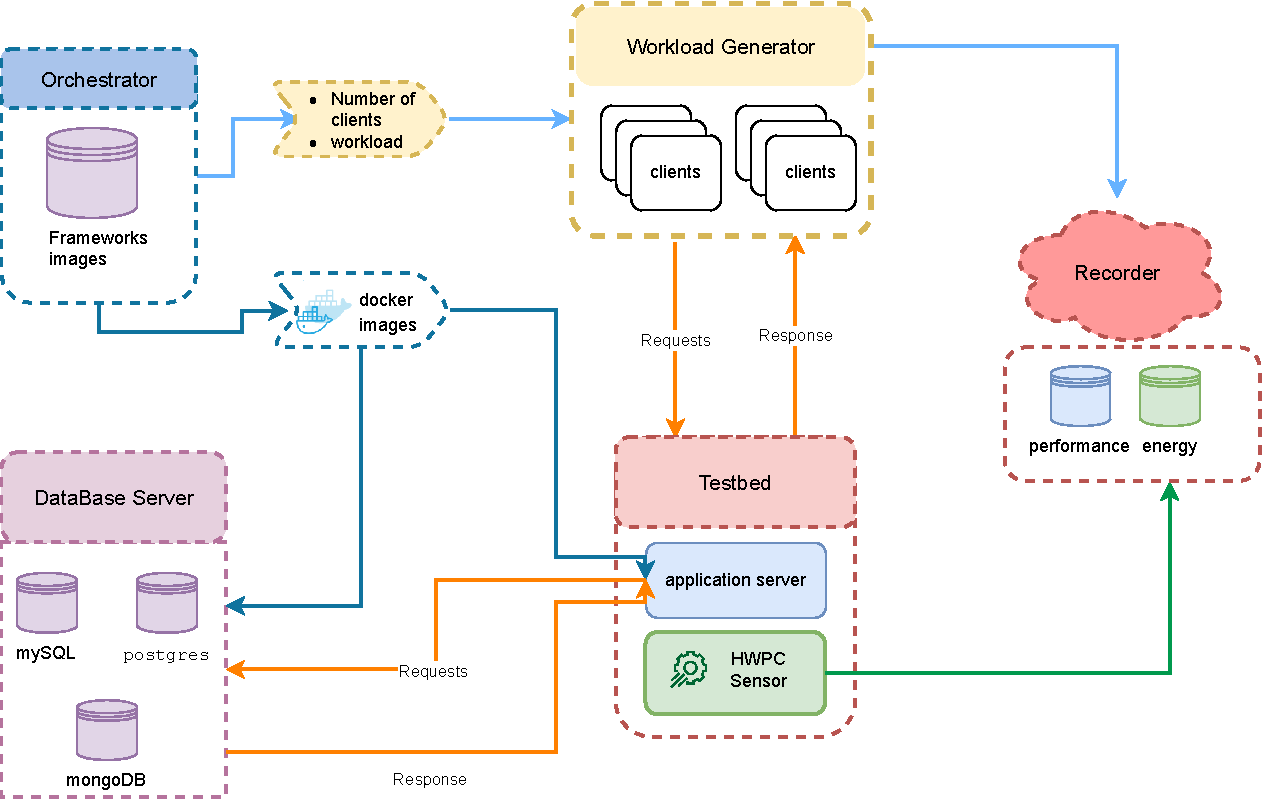
\includegraphics[width=.8\columnwidth]{imgs/architecture}
    \caption[Architecture]{Architecture of the experiments.}
    \label{fig:architecture}
\end{figure}


\paragraph{Bias Analysis}
We are aware of potential bias analysis regarding the estimation of the total energy cost, the interference of other system processes during the execution and some external events.
Thus, we run experiments multiple times and compute the average values.

\subsubsection{Extension}
To follow the guidelines that we presented in Chapter~\ref{chapter:benchmarking}, we provide a GitHub repository\footnote{\url{https://github.com/chakib-belgaid/FrameworkBenchmarks}} where one can add extra \textbf{candidates} by creating a new project using the option \texttt{--new}.
Then, interested practitioners have to fill the template and provide the Docker image file.
Additionally, to configure the \textbf{workload} we provide the option \texttt{--concurrency-levels} and \texttt{--duration}.
The choice of the database is included in the Docker image.

\subsection{Results \& Findings}
Overall we had $8,750$ benchmarks, and all can be found in the online repository.\footnote{\url{https://github.com/chakib-belgaid/frameworks-benchmarks-results}}
In this section, we discuss these results to answer the following questions:
\begin{itemize}
    \item is there a dominating programming language when it comes to performance, energy consumption, and latency?
    \item which class of programming language is performing well?
    \item is there a correlation between energy consumption and latency?
    \item is there an impact on the server when it comes to changing the database?
\end{itemize}

Since most of the companies use the same stack, we do not aggregate the results as it may lead to confusion.
For example, comparing the average energy consumption of each programming language will not reflect reality, particularly when we have two web frameworks at the opposite ends of the spectrum.

\subsubsection{Overall Statistics}
% To determine which web framework/stack is performing wellm we need to establish some general idea about the average.
To determine which web framework/stack is performing well, we need to establish some general idea about the average energy consumption and latency of the frameworks under study.
Instead of reporting the raw energy consumption of those frameworks, we will provide some green factors to determine which one is eco-friendly and which one is greedy.
In this part, we will discuss the average behavior of the frameworks, highlight some trends, and eliminate the outliers.
As we said in the threats to validity, being an outlier in this case does not mean that the web framework is not performing well, it means that the web framework is not performing well in the same way as the others within the context of this experiment.

On the other hand, the cost of a single request is proportional to the number of requests per second of the web framework.
To narrow the research space, we will look for a correlation between the metrics.
The Pearson correlation coefficient~\cite{zar2005spearman} will be used to determine this correlation.
Because the Shapiro-Wilk~\cite{shapiro1968comparative} test yielded a $p$-value of 0.0 for all metrics.
% TODO : REPHRASE THIS SENTENCE
\begin{figure}[htb]
    \centering
    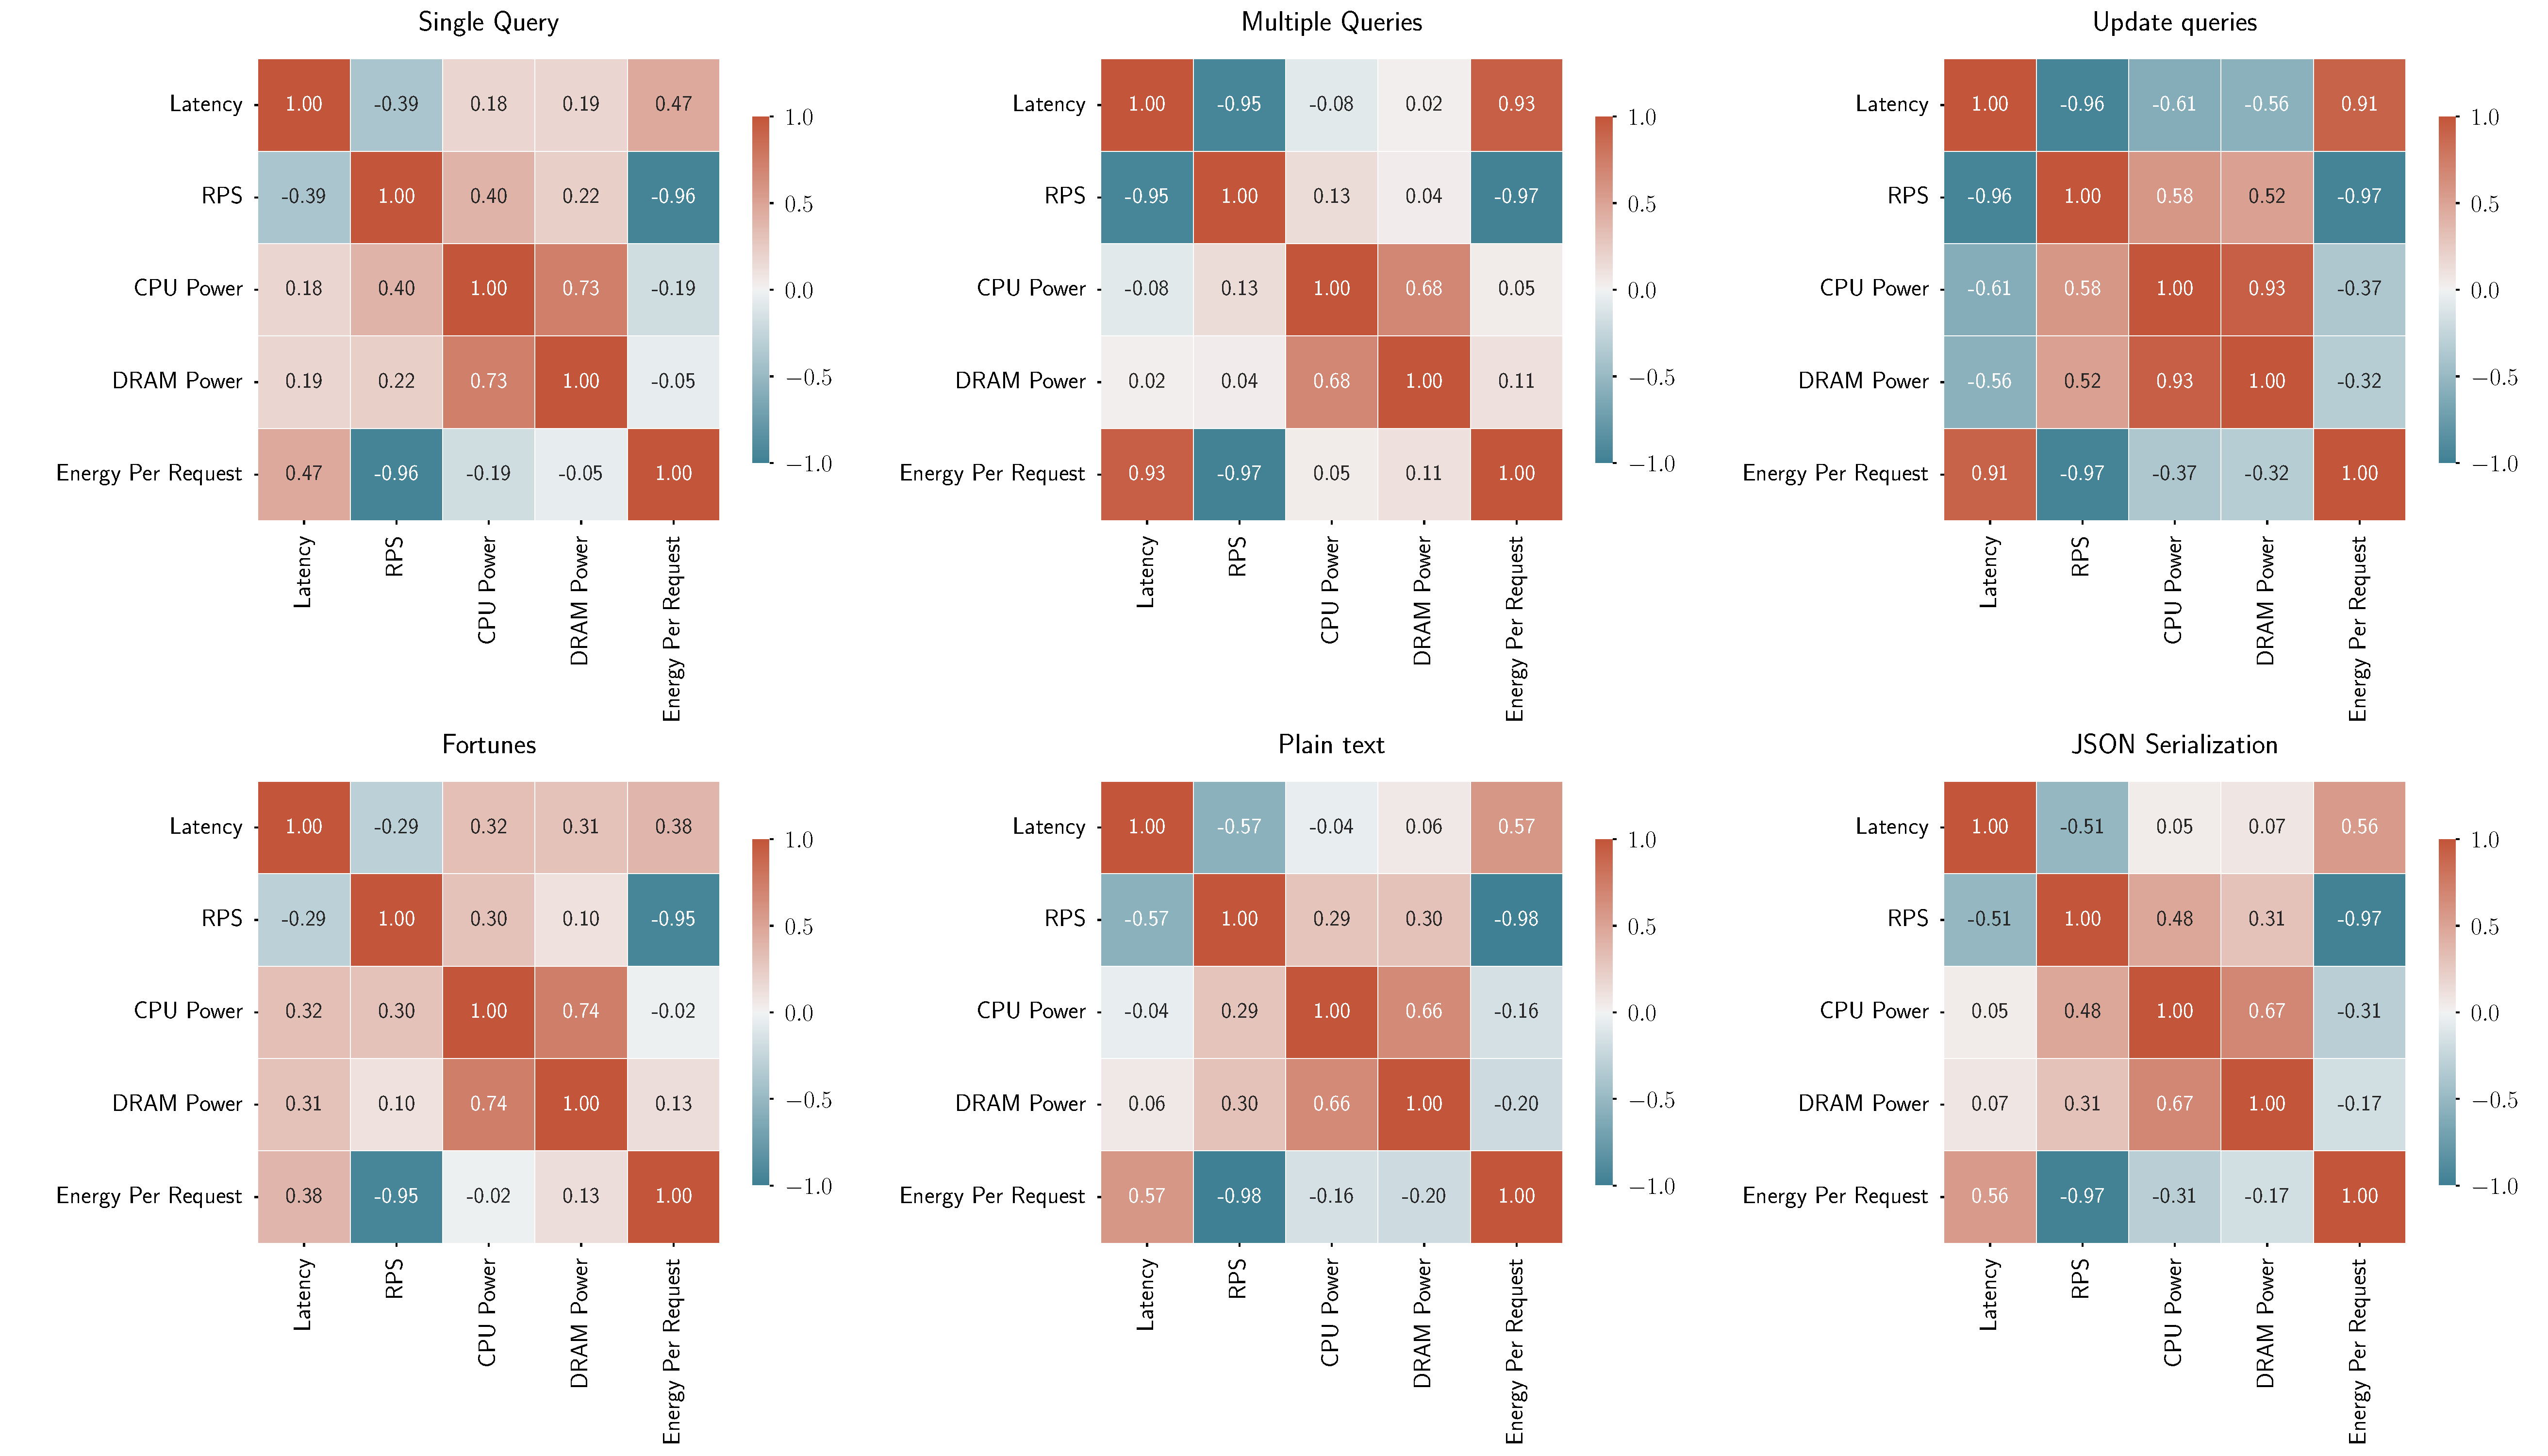
\includegraphics[width=\textwidth]{imgs/correlation_all}
    \caption{Spearman Rank Correlation between different metrics}
    \label{fig:correlation}
\end{figure}

Figure~\ref{fig:correlation} depicts the correlation between the metrics for the 6 scenarios.
The Pearson correlation coefficient quantifies the linear correlation between two variables X and Y.
It ranges from -1 to +1, with 1 being total positive linear correlation, 0 representing no linear correlation, and -1 representing whole negative linear correlation.
The stronger the correlation, the closer the value is to 1 or -1.
The weaker the correlation, the closer the value is to zero.
The Pearson product-moment correlation coefficient is another name for the correlation coefficient.
This correlation coefficient is also known as the Pearson product-moment correlation coefficient.
One can notice that there is a strong correlation between the energy consumption of the CPU and the DRAM for most of the scenarios.
Moreover the average energy consumption of DRAM is one sixth of the CPU energy consumption.
Therefore, in this study we will focus more on the CPU energy consumption.
For more insights about the DRAM consumption we refer the reader to our github repository.\footnote{\url{https://github.com/chakib-belgaid/frameworks-benchmarks-results}}

Another strong correlation is between the number of requests per second and the average cost of a single request.
This is because the cost a single request is proportionate to the number of requests per second of the framework, since the Average Power consumption remains constant after a certain threshold of clients.

Unlike the \emph{multiple queries and update} queries, another scenario depicts a weak correlation between latency and number of requests per second.
The reason behind such an anomaly is the fact that we summarized the data when we had a multiple number of clients.
If we calculate the correlation when we have a fixed number of client, like the case of update queries (512 clients), one can notice a strong correlation.

\begin{figure}[bht]
    \centering
    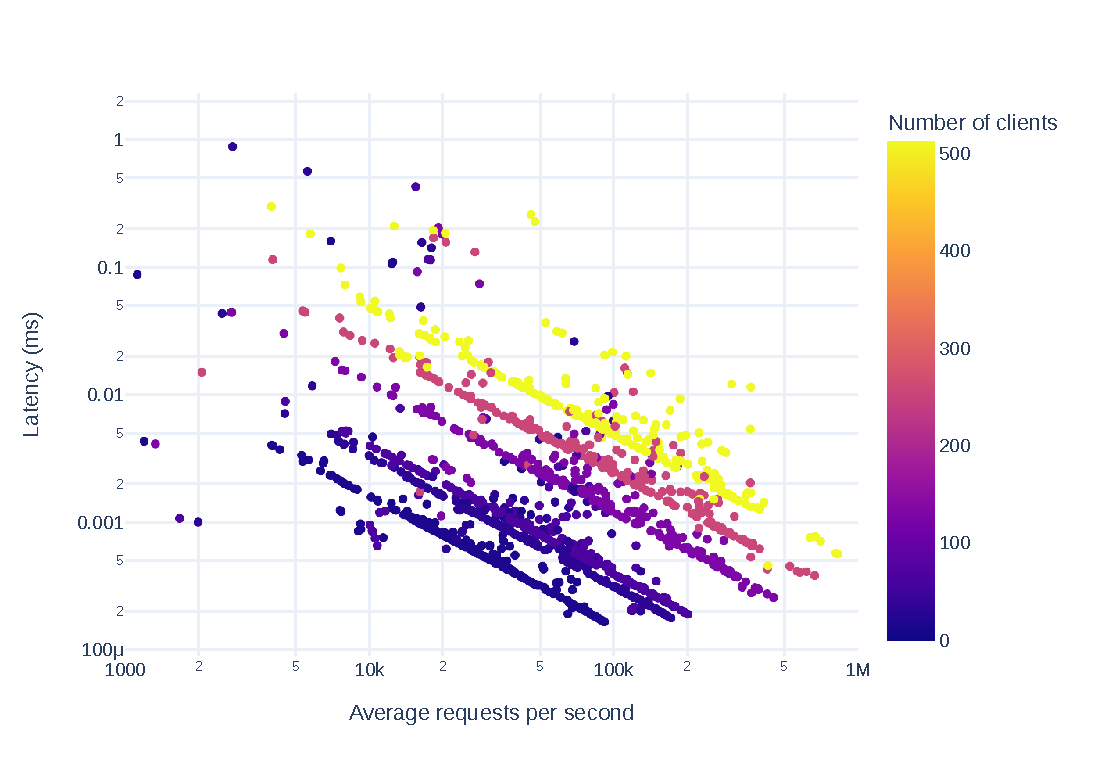
\includegraphics[width=.9\columnwidth ]{imgs/scatter_db_latency_rps}
    \caption{Correlation of latency and number of requests per second for a single query}
    \label{fig:scatter_db}
\end{figure}

Figure~\ref{fig:scatter_db} demonstrates such a behavior.
As one can notice, for each level we observe a linear clustering.
Therefore, we can safely focus our analysis on two variables, \emph{number of requests per second} and \emph{average energy consumption}.
The first one will indicate the performance of the solution meanwhile the second one will be used to measure how green a framework is.

\begin{figure}[bht]
    \centering
    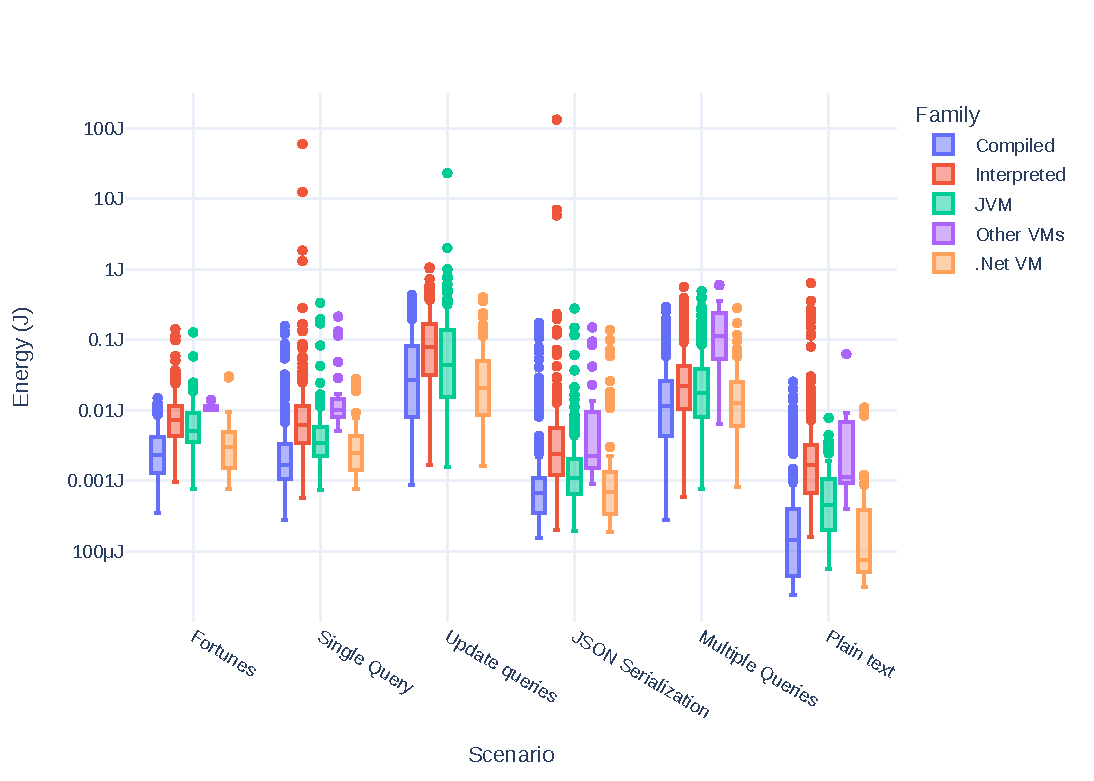
\includegraphics[width=.9\columnwidth ]{imgs/all_boxplot}
    \caption{Energy consumption per request for each family of programming languages}
    \label{fig:all_boxplot}
\end{figure}
%  THIS might be completely changed , i think we need to check the limits of the data base 


% intersently there is no correlation between the energy consumption of the CPU and the latency, which means that we can achieve both a low latency and a low energy consumption at the same time. 


\subsubsection{Scenario-based Analysis}
This section will focus on the behavior of all the implementations for each scenario.
For visibility purposes, we will group the frameworks not by language but by family, so we will have 5 families:
\begin{itemize}
    \item \textbf{compiled languages}: Rust, C, GO and C++;
    \item \textbf{interpreted languages}: Python, PHP and Javascript;
    \item \textbf{JVM-based languages}: Java, Kotlin, Scala and Clojure;
    \item \textbf{.Net-based languages}: C\#, F\# and VB;
    \item \textbf{Other VM-based languages}: Dart and Elixir.
\end{itemize}

Figure~\ref{fig:all_boxplot} depicts the programming language and the family for each framework.

\paragraph{Idle behviour}
This part will treat average power behavior when the framework is in a rest mode.
Figure~\ref{fig:av_power_idle} presents, a density plot for each family.

\begin{figure}[bht]
    \centering
    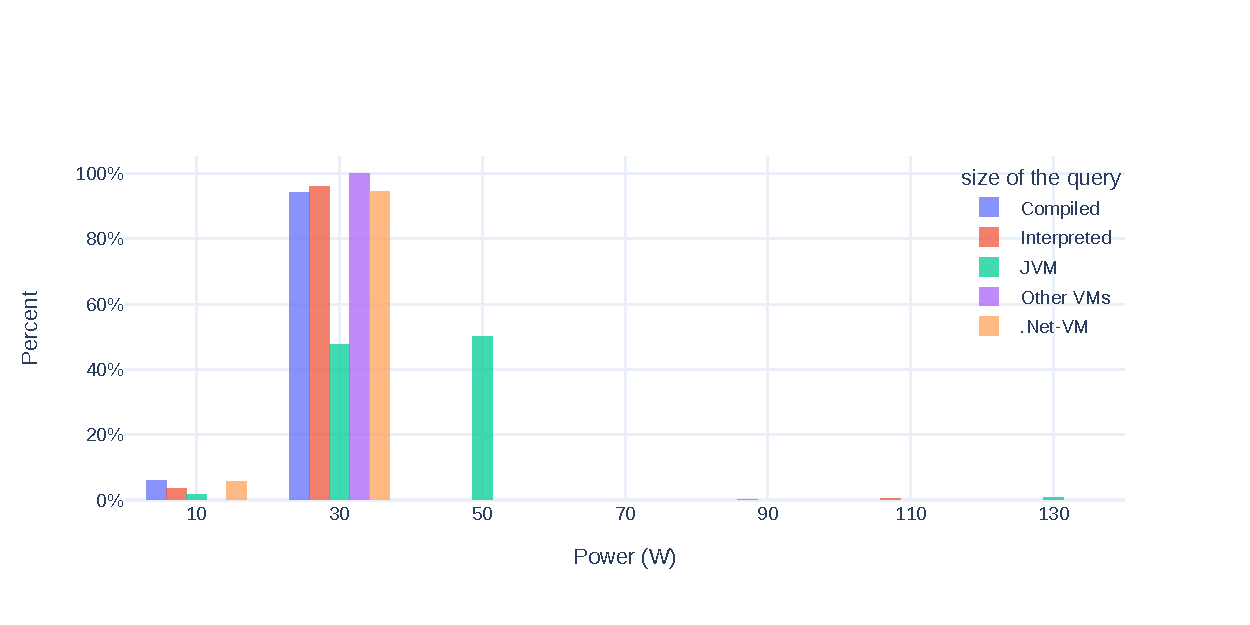
\includegraphics[width=1.0\columnwidth]{imgs/av_power_idle}
    \caption{Average power consumption for the idle scenario}
    \label{fig:av_power_idle}
\end{figure}

As one can notice at rest, most of the families consumes between 20 and 40 Watts, 6\% of the compiled languages frameworks consumes less than 15 Watts.
However, 50\% of Java solutions tend to consume around 50 Watts, which makes it the most greedy family.
If we look at the each of the programming languages from Java, separately in Figure~\ref{fig:av_power_java_idle}, we find that Java-based implementations tend to consume around 50 Watts, while Kotlin, Clojure and Scala consume around 30 Watts.

\begin{figure}[bht]
    \centering
    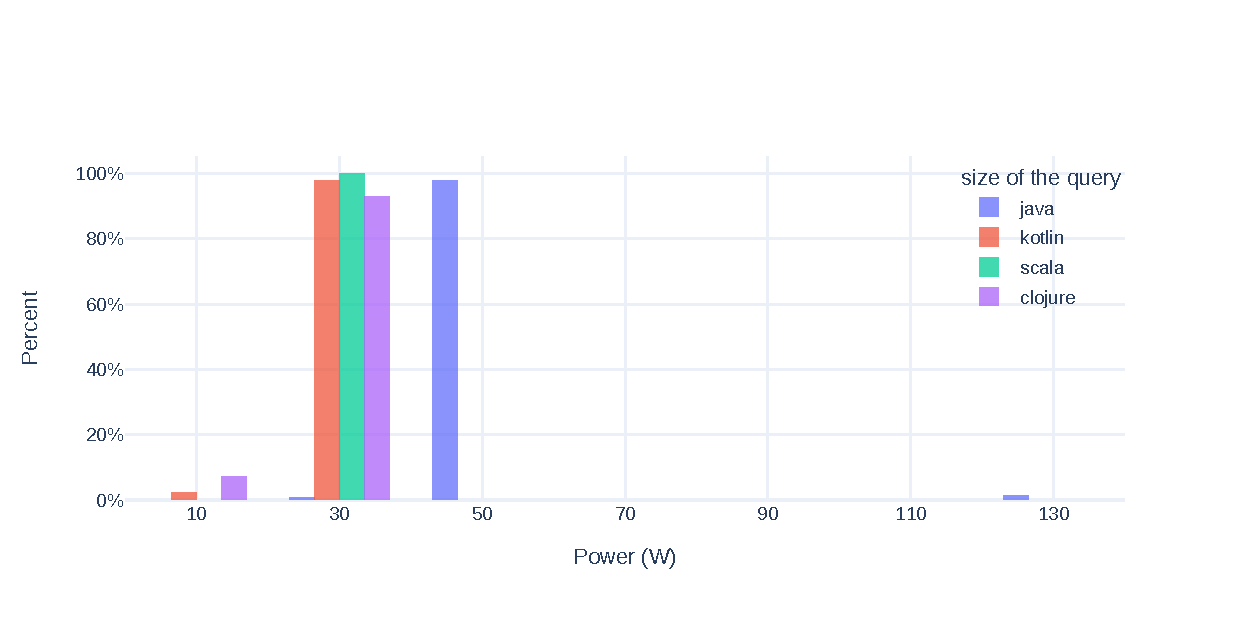
\includegraphics[width=1.0\columnwidth]{imgs/av_power_java_idle}
    \caption{Average power consumption for Java-based languages in the idle scenario case}
    \label{fig:av_power_java_idle}
\end{figure}

\paragraph{Single query}
As mentioned before, the purpose of this scenario is to benchmark the framework efficiency to handle a single entry.
To determine the general behavior of the frameworks, first we will start with an histogram of average power consumption.
Figure~\ref{fig:av_power_db} reports on the  density plot of average power consumptions for all the experiments depending on the number of concurrent clients.
As one can observe, there are three main states:
\begin{enumerate}
    \item \emph{relaxed state} where the number of clients is less than 16: most of the frameworks consumes around 70 Watts;
    \item \emph{average state} where the number of clients is between 16 and 64: most of the frameworks consumes around 100 Watts;
    \item Finally the \emph{stress state} beyond 128 concurrent clients: most of the frameworks  have a stable power consumption regardless of the number of clients.
    This is due to database server, which reached its maximum capacity.
\end{enumerate}

\begin{figure}[hbt]
    \centering
    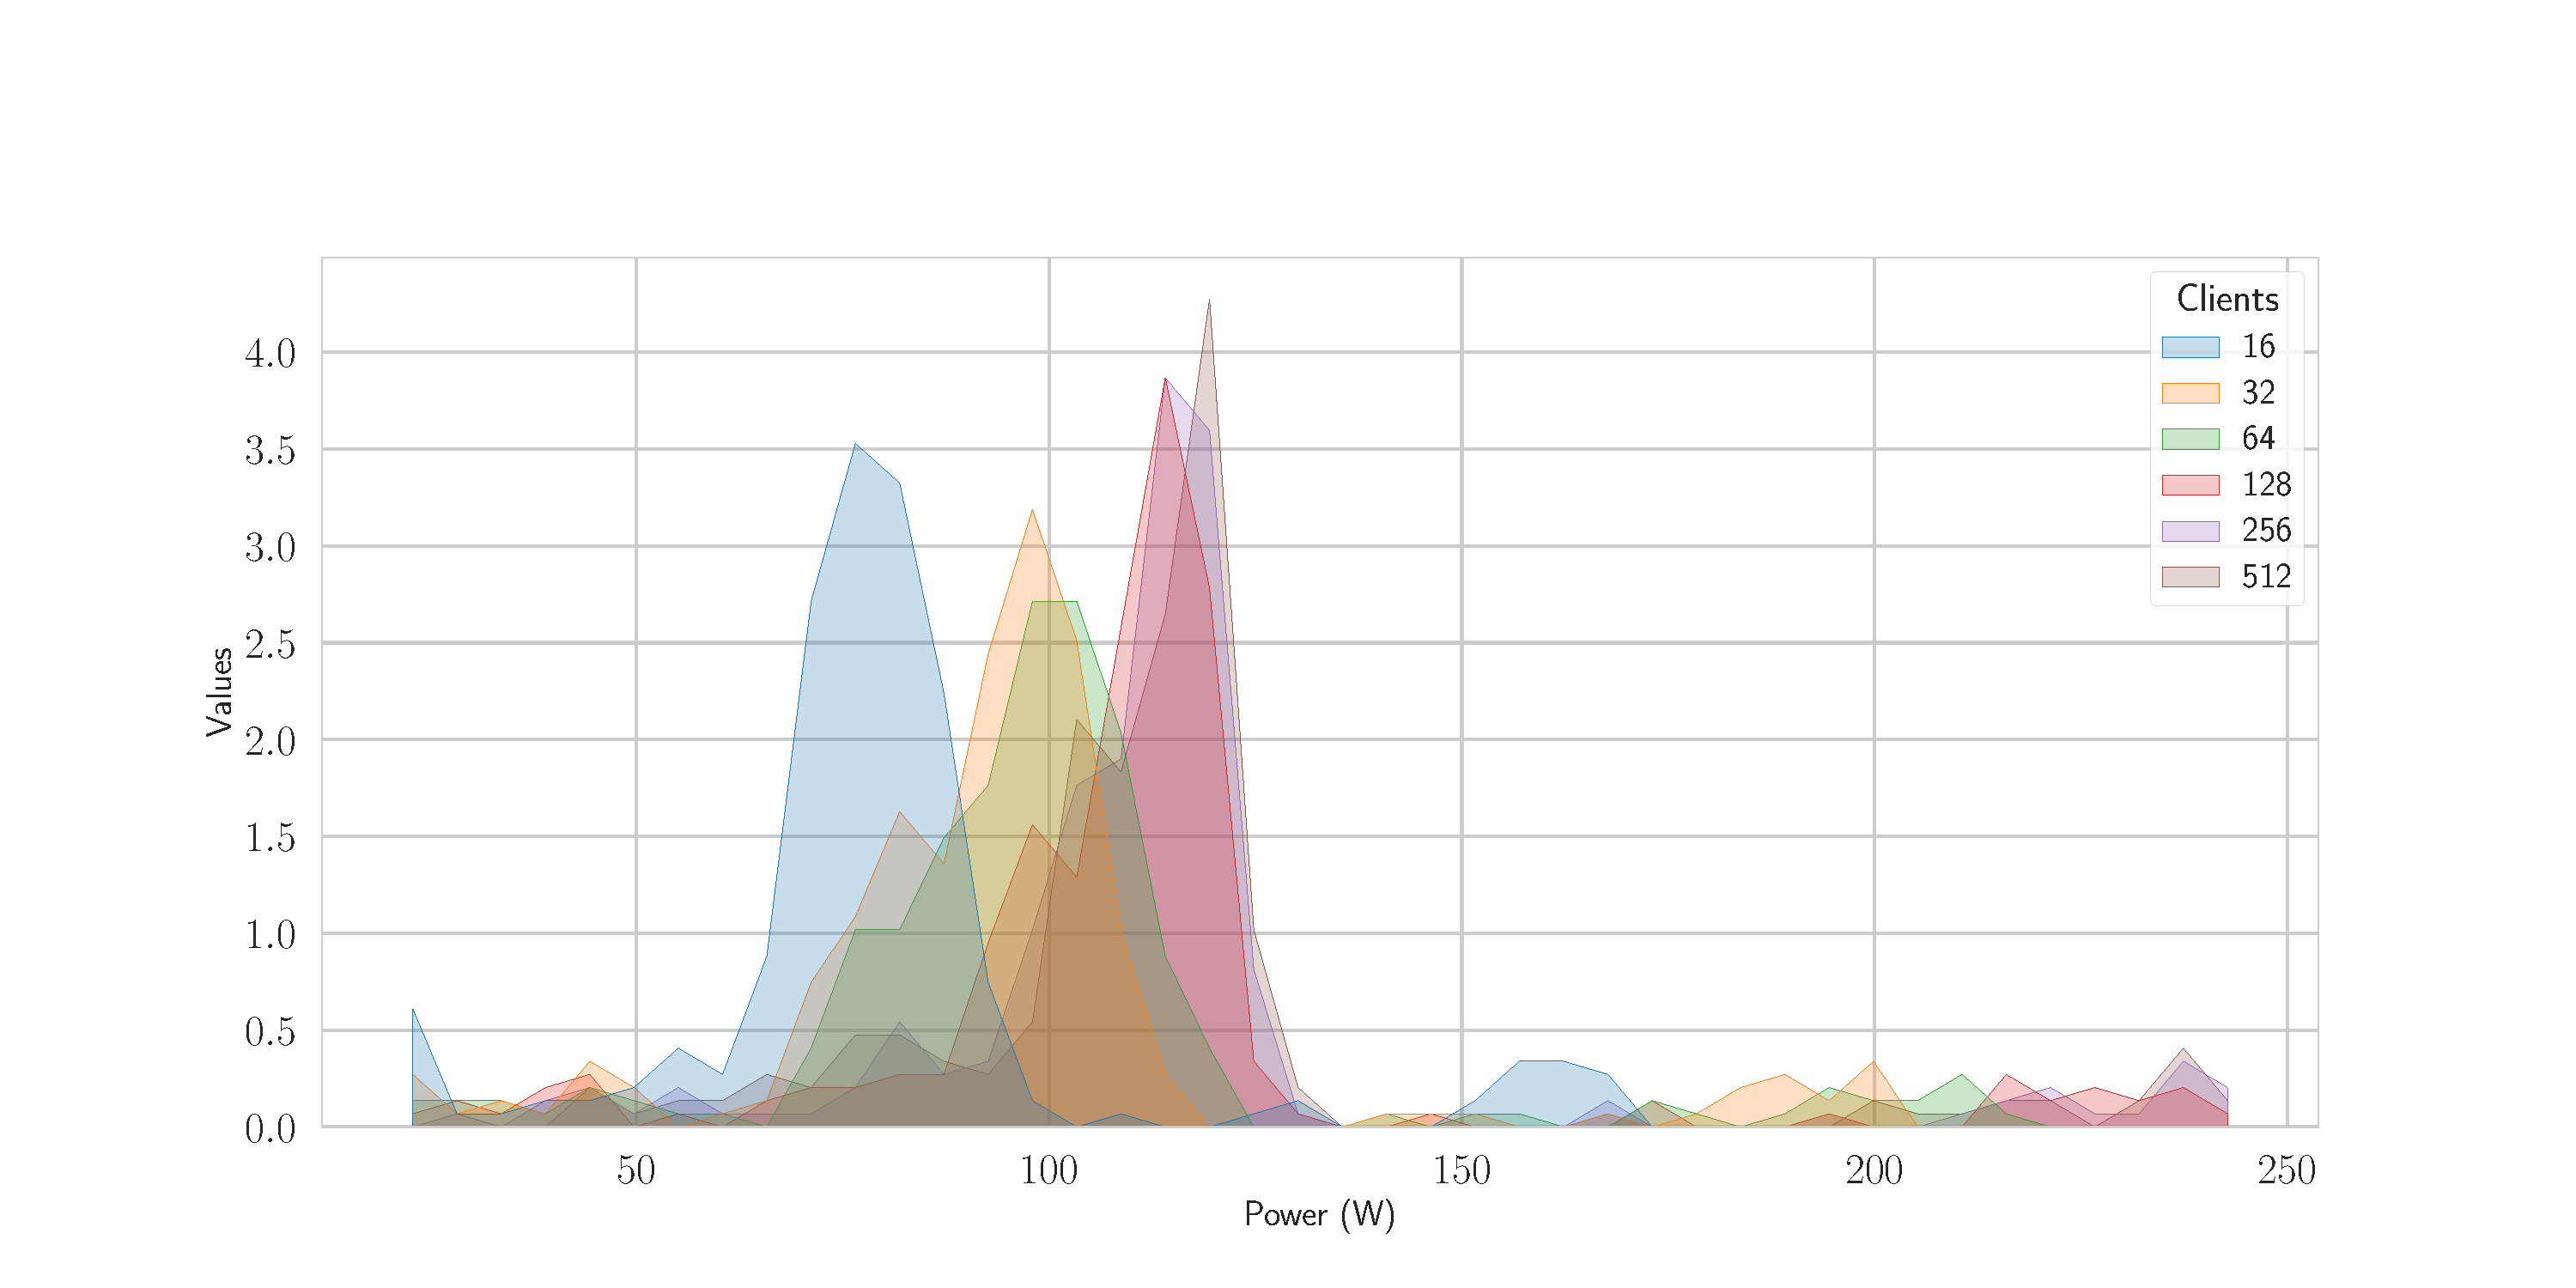
\includegraphics[width=\textwidth,height=\textheight,keepaspectratio]{imgs/histogram_av_power_cpu_db}
    \caption{Average power consumption for the Single query test }
    \label{fig:av_power_db}
\end{figure}

Now that we have seen the overall distribution of the power within the single query scenario.
We analyze each family separately.
In addition to that, we include the number of \emph{requests per second} (RPS) as a performance metrics of interest.
In Figure~\ref{fig:power_requests_db}, each run is represented by a circle, and the size of the circle represents the number of concurrent clients: The smaller the circle the less clients.
On the one hand, one can notice that compiled languages are the most efficient in terms of performance, despite their low energy consumption.
Moreover, there is no significant change in the average power consumption when we increase the number of concurrent clients.
On the other hand, the JVM-based frameworks tend to consume the most energy while reporting the same performance as the .Net-based ones.
Finally, the interpreted languages lack in terms of performance while keeping low average power, except for PHP, as it is has one of the highest RPS with a half million RPS which got beaten only by C++ and Rust.

\begin{figure}[hbt]
    % \centering
    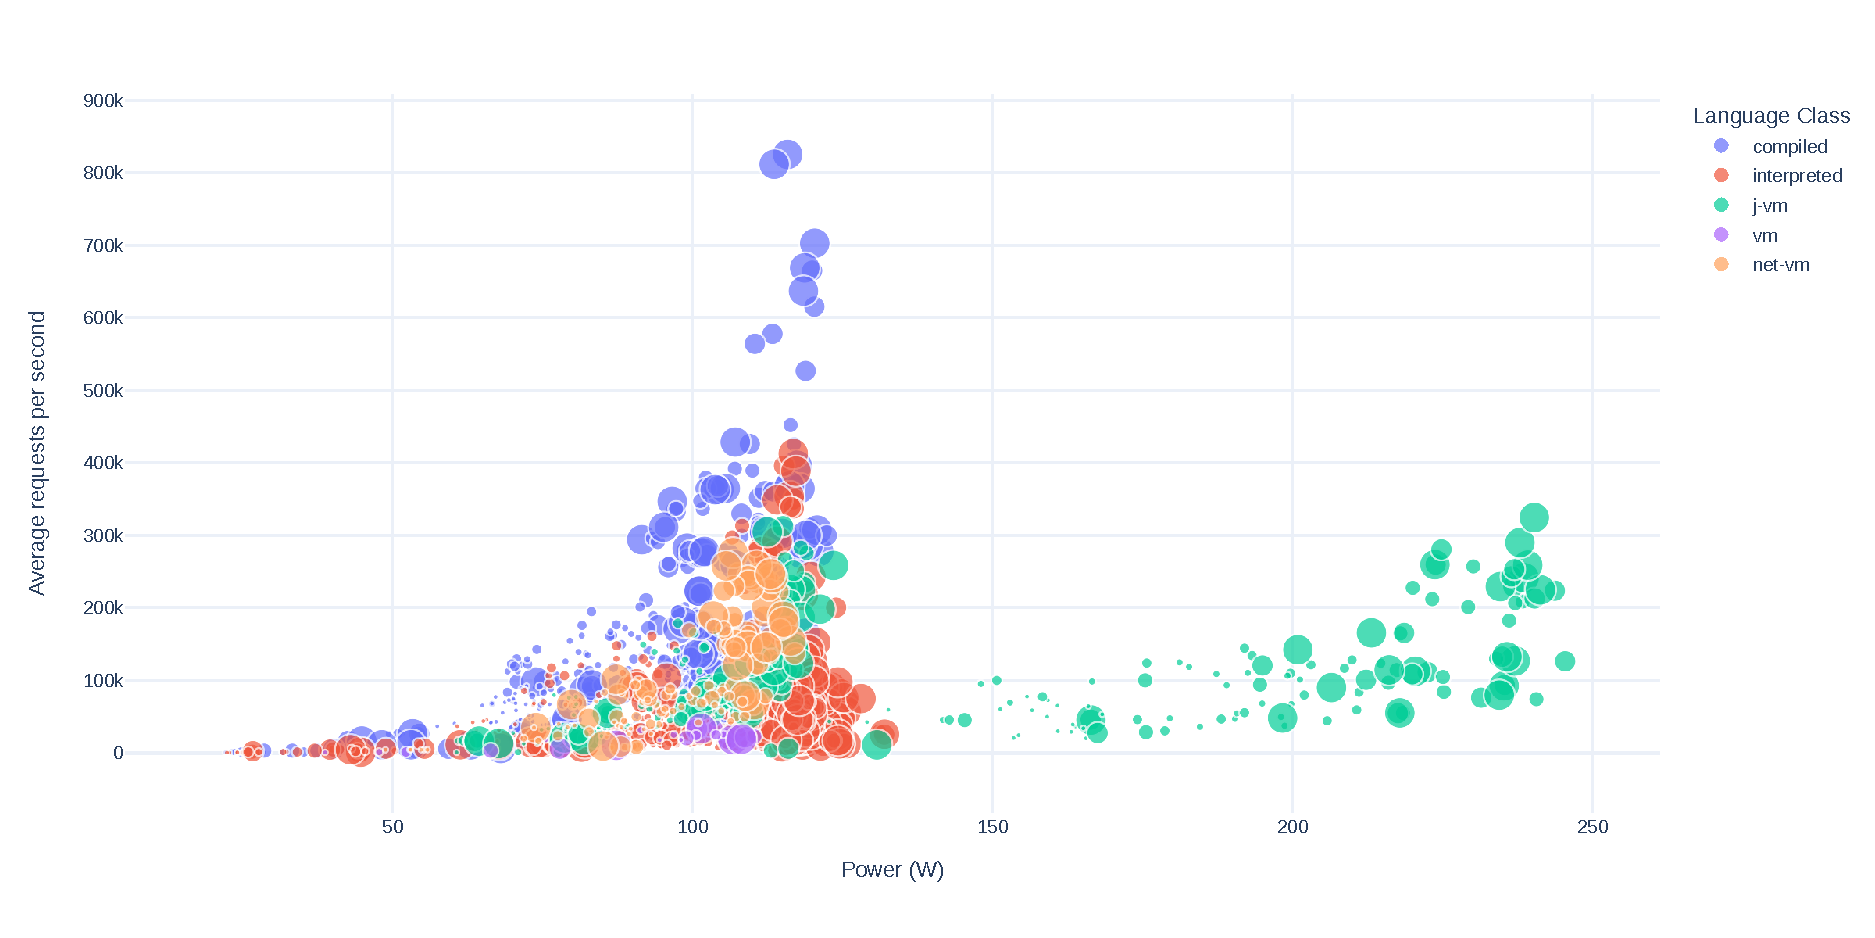
\includegraphics[height=\textwidth,width=\textheight,keepaspectratio,angle=90]{imgs/power_requests_db}
    \caption{Total request Vs average power consumption for the \emph{single query} benchmark (size of circles represents the number of clients)}
    \label{fig:power_requests_db}
\end{figure}

\paragraph{Multiple queries}
This scenario is used to benchmark the framework efficiency to handle multiple row queries.
As mentioned before, this study focuses on a fixed number of concurrent clients while we increase the size of the request per level.
Figure~\ref{fig:av_power_query} reports on the average power consumption for each level.
As one can notice, the size of the query has no strong impact on the average power consumption.
Furthermore, one can notice a slight decrease in the average power consumption (from 110 watts to 90 watts) when the size is bigger than 10 rows.
This might be related to the time taken by the database to process the query.
Therefore, one can conclude that the size of the query has more impact on the database than the framework itself.

\begin{figure}[hbt]
    \centering
    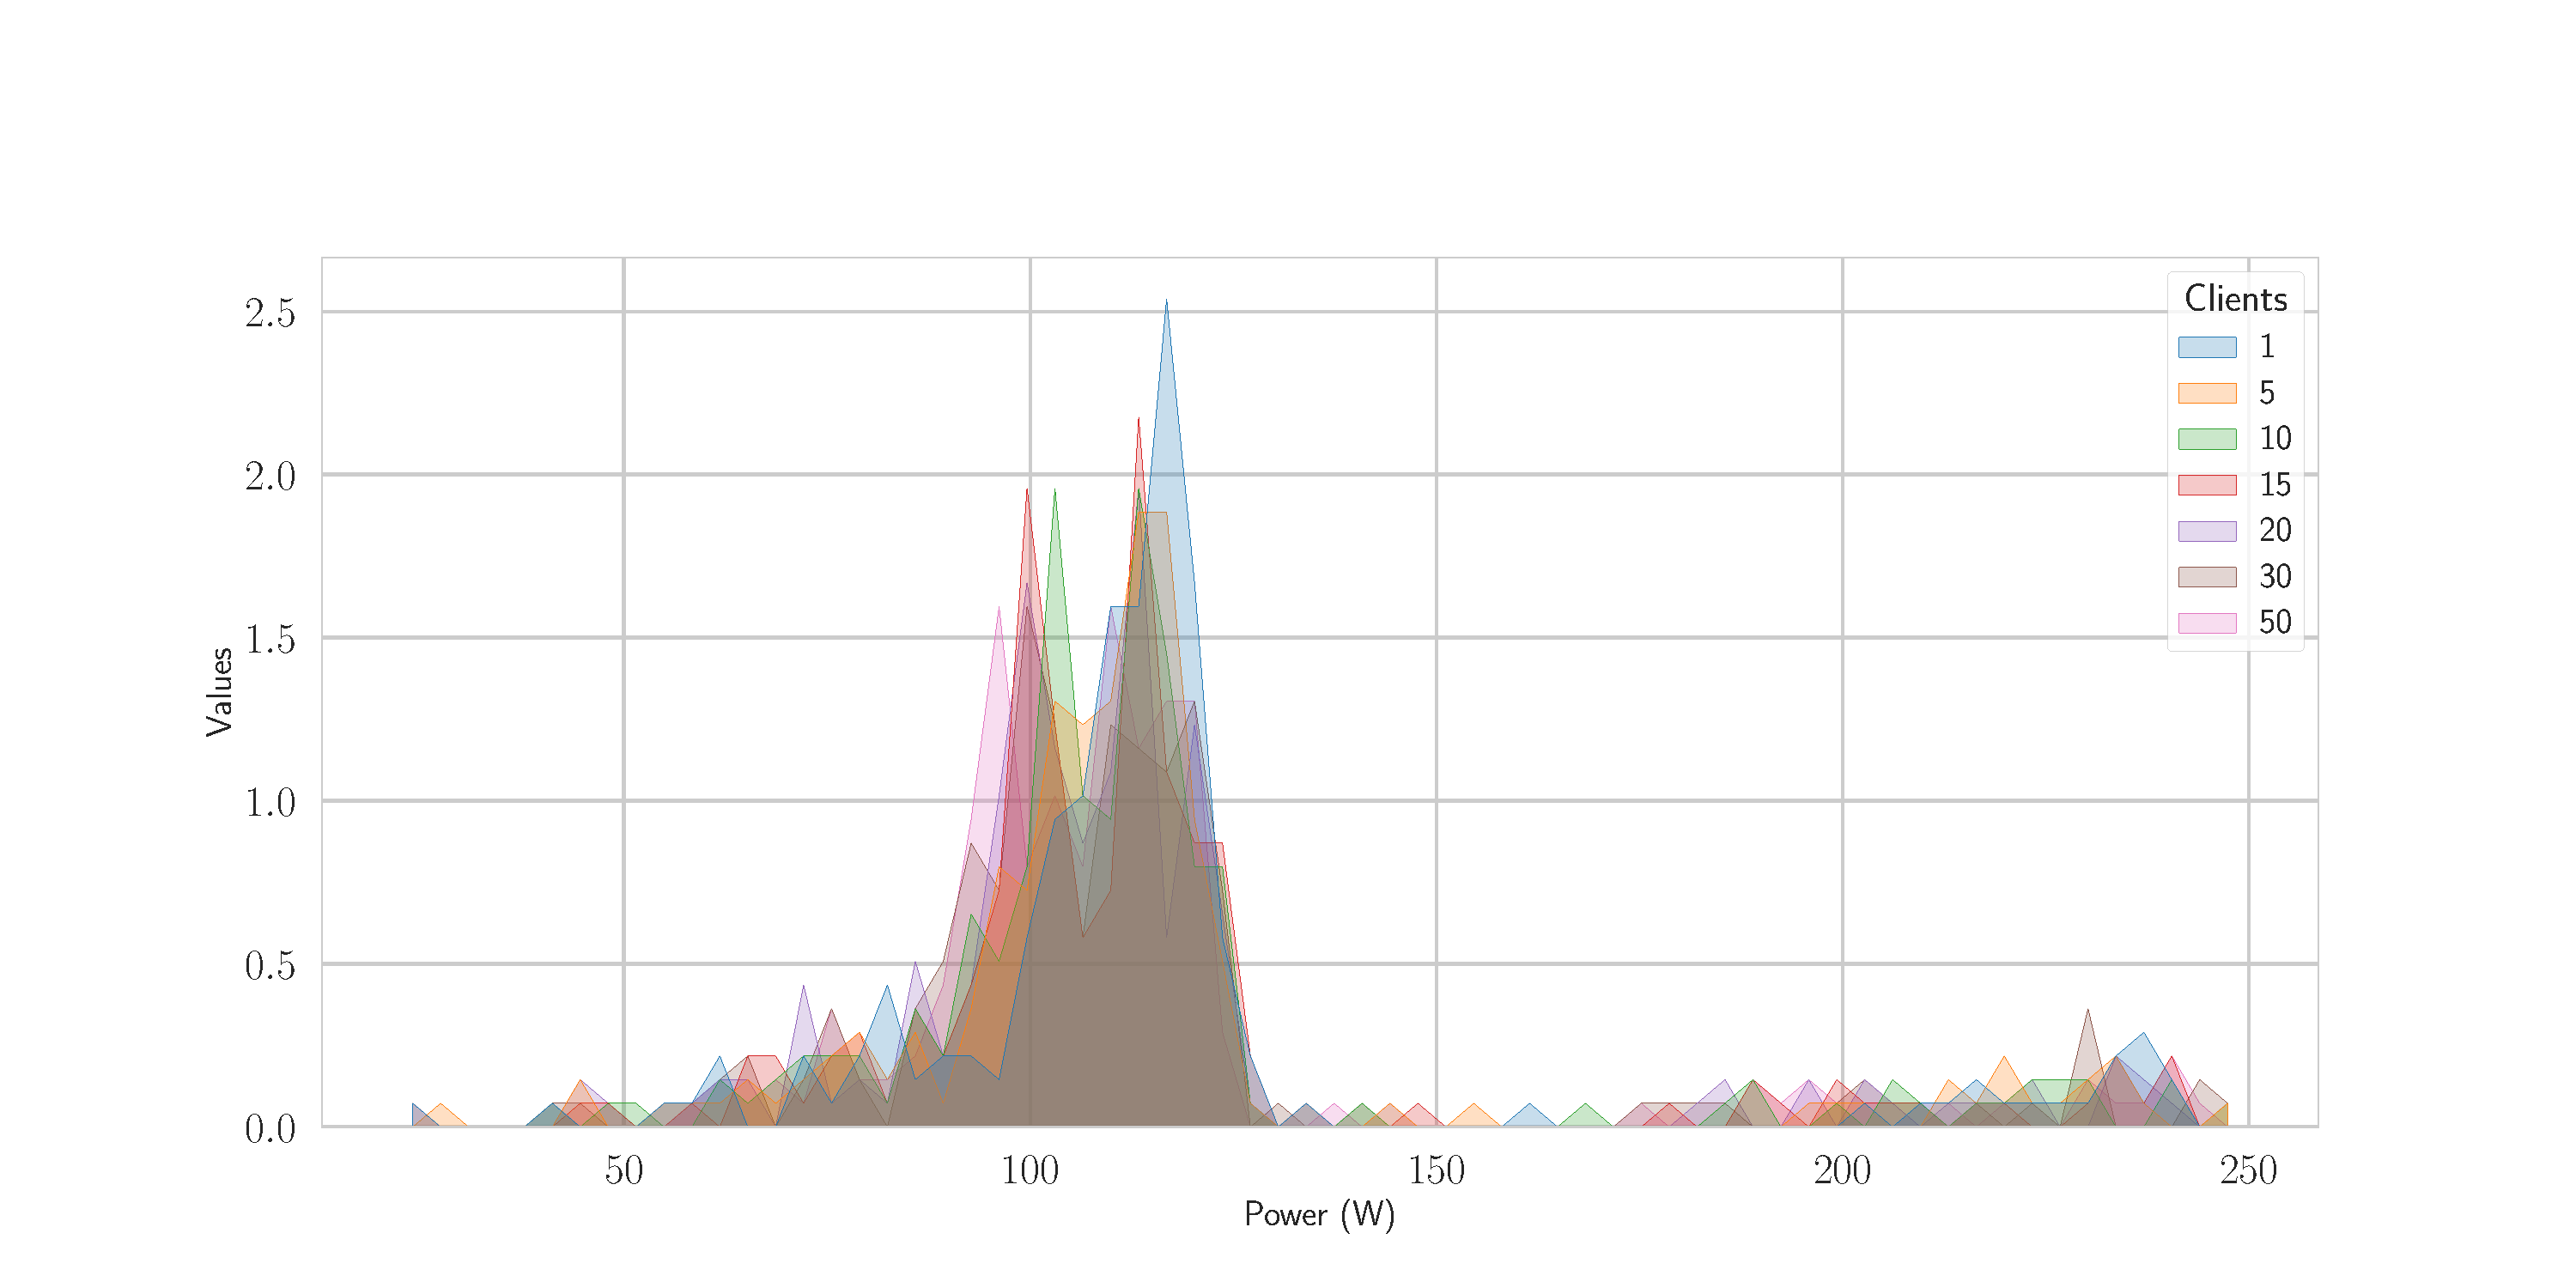
\includegraphics[width=\textwidth,height=\textheight,keepaspectratio]{imgs/histogram_av_power_cpu_query}
    \caption{Average power consumption for the multiple queries }
    \label{fig:av_power_query}
\end{figure}

Table~\ref{table:query_db_row} details the average power consumption per level for each database.
One can see, that for MySQL there were no changes regardless of the size of the query, while for Postgres and MongoDB there is a slight decrease in the average power consumption when the size of the query is bigger than 10 rows.
%  should add into perspective to study the energy consumption of the data base server itself 

\begin{table*}[bth]
    \raggedright
    \caption{Average power consumption of frameworks based on the database type}
    \label{table:query_db_row}
    \resizebox{\textwidth}{!}{
        \begin{tabular}{l|c|c|c|c|c|c|c|}
            \toprule
            \textbf{Query size} & 1      & 5      & 10     & 15     & 20     & 30     & 50     \\
            \hline
            MongoDB             & 97.17  & 96.93  & 93.38  & 92.58  & 91.61  & 92.585 & 91.17  \\
            MySQL               & 113.86 & 112.92 & 112.74 & 113.05 & 112.13 & 112.62 & 112.16 \\
            PostgresSQL         & 113.86 & 108.25 & 106.19 & 102.97 & 103.41 & 101.95 & 102.96 \\
            \bottomrule
        \end{tabular}}
\end{table*}

Now that we have seen the overall distribution of power within the multiple query scenario, we can analyze each family separately.
We consider the number of requests per second (aka RPS) as related performance metrics. 
Figure~\ref{fig:power_requests_query} presents the total RPS per level for each framework in a logarithmic scale.
As one can notice, the difference between the best performing framework, aka Lithium,\footnote{\url{https://matt-42.github.io/lithium/}} and the worst one, aka hapi-nginx,\footnote{\url{https://github.com/hapijs/hapi}} is $4,000$ times, while the average in power consumption is 5 times (120 for lithium vs 25 for hapi).
This highlight the importance of target scale of the application when choosing the framework.
Java-based frameworks tend to consume more power compared to other languages with a slight increase in performance.
PHP remains one of the most efficient frameworks in terms of performance, while keeping low average power consumption.

\begin{figure}[hbt]
    % \centering
    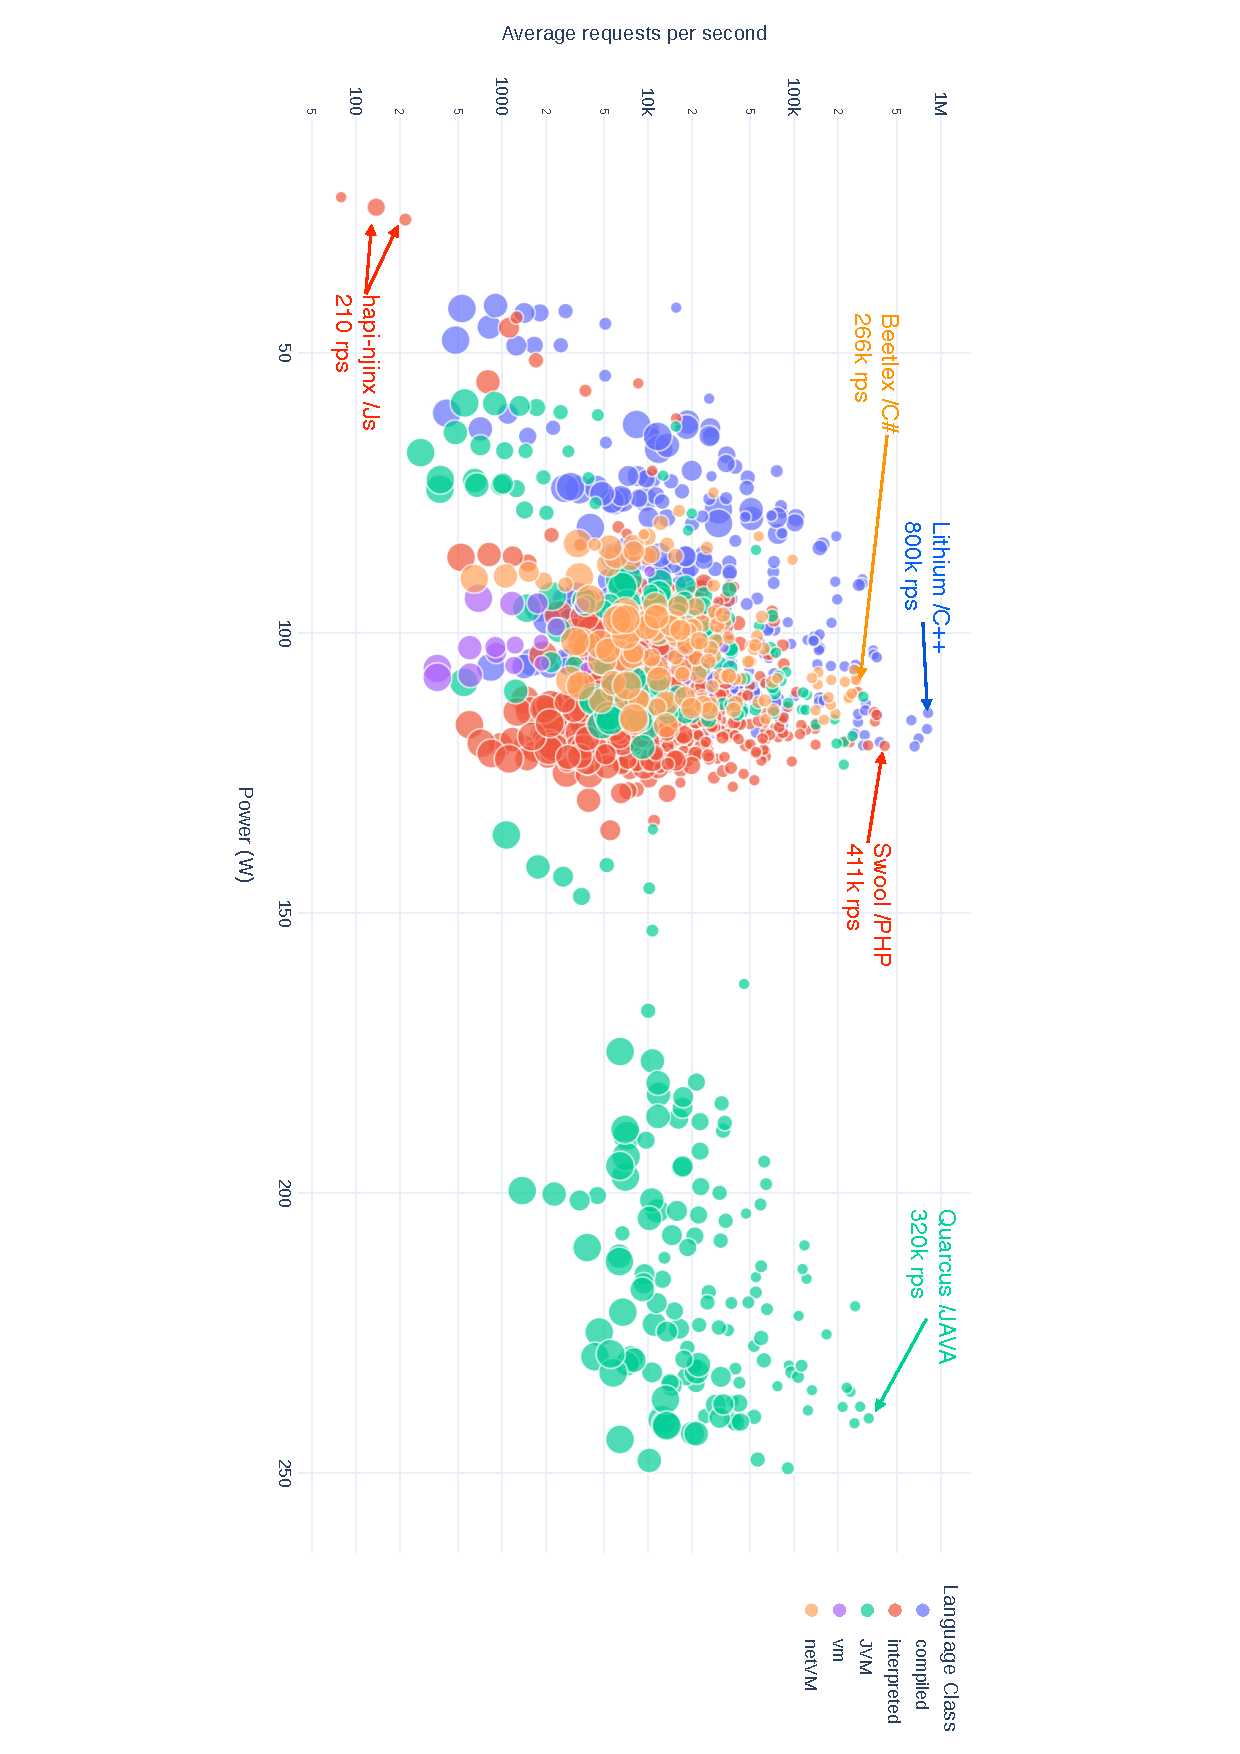
\includegraphics[height=\textwidth,width=\textheight,keepaspectratio,angle=90]{imgs/power_requests_query_log}
    \caption{Total request vs average power consumption for the single query benchmark (size of circles represents the number of clients) }
    \label{fig:power_requests_query}
\end{figure}

\paragraph{Update}
This scenario benchmark the framework efficiency to handle update queries.
As mentioned before, for this study we will focus on the a fixed number of parallel clients while we increase the size of the request per each level.
Figure~\ref{fig:av_power_update} presents the average power consumption for each level.
As one can notice, the size of the query has not a strong impact on the average power consumption.
Moreover, the overall average power consumption decreased by 20 Watts.

\begin{figure}[hbt]
    \centering
    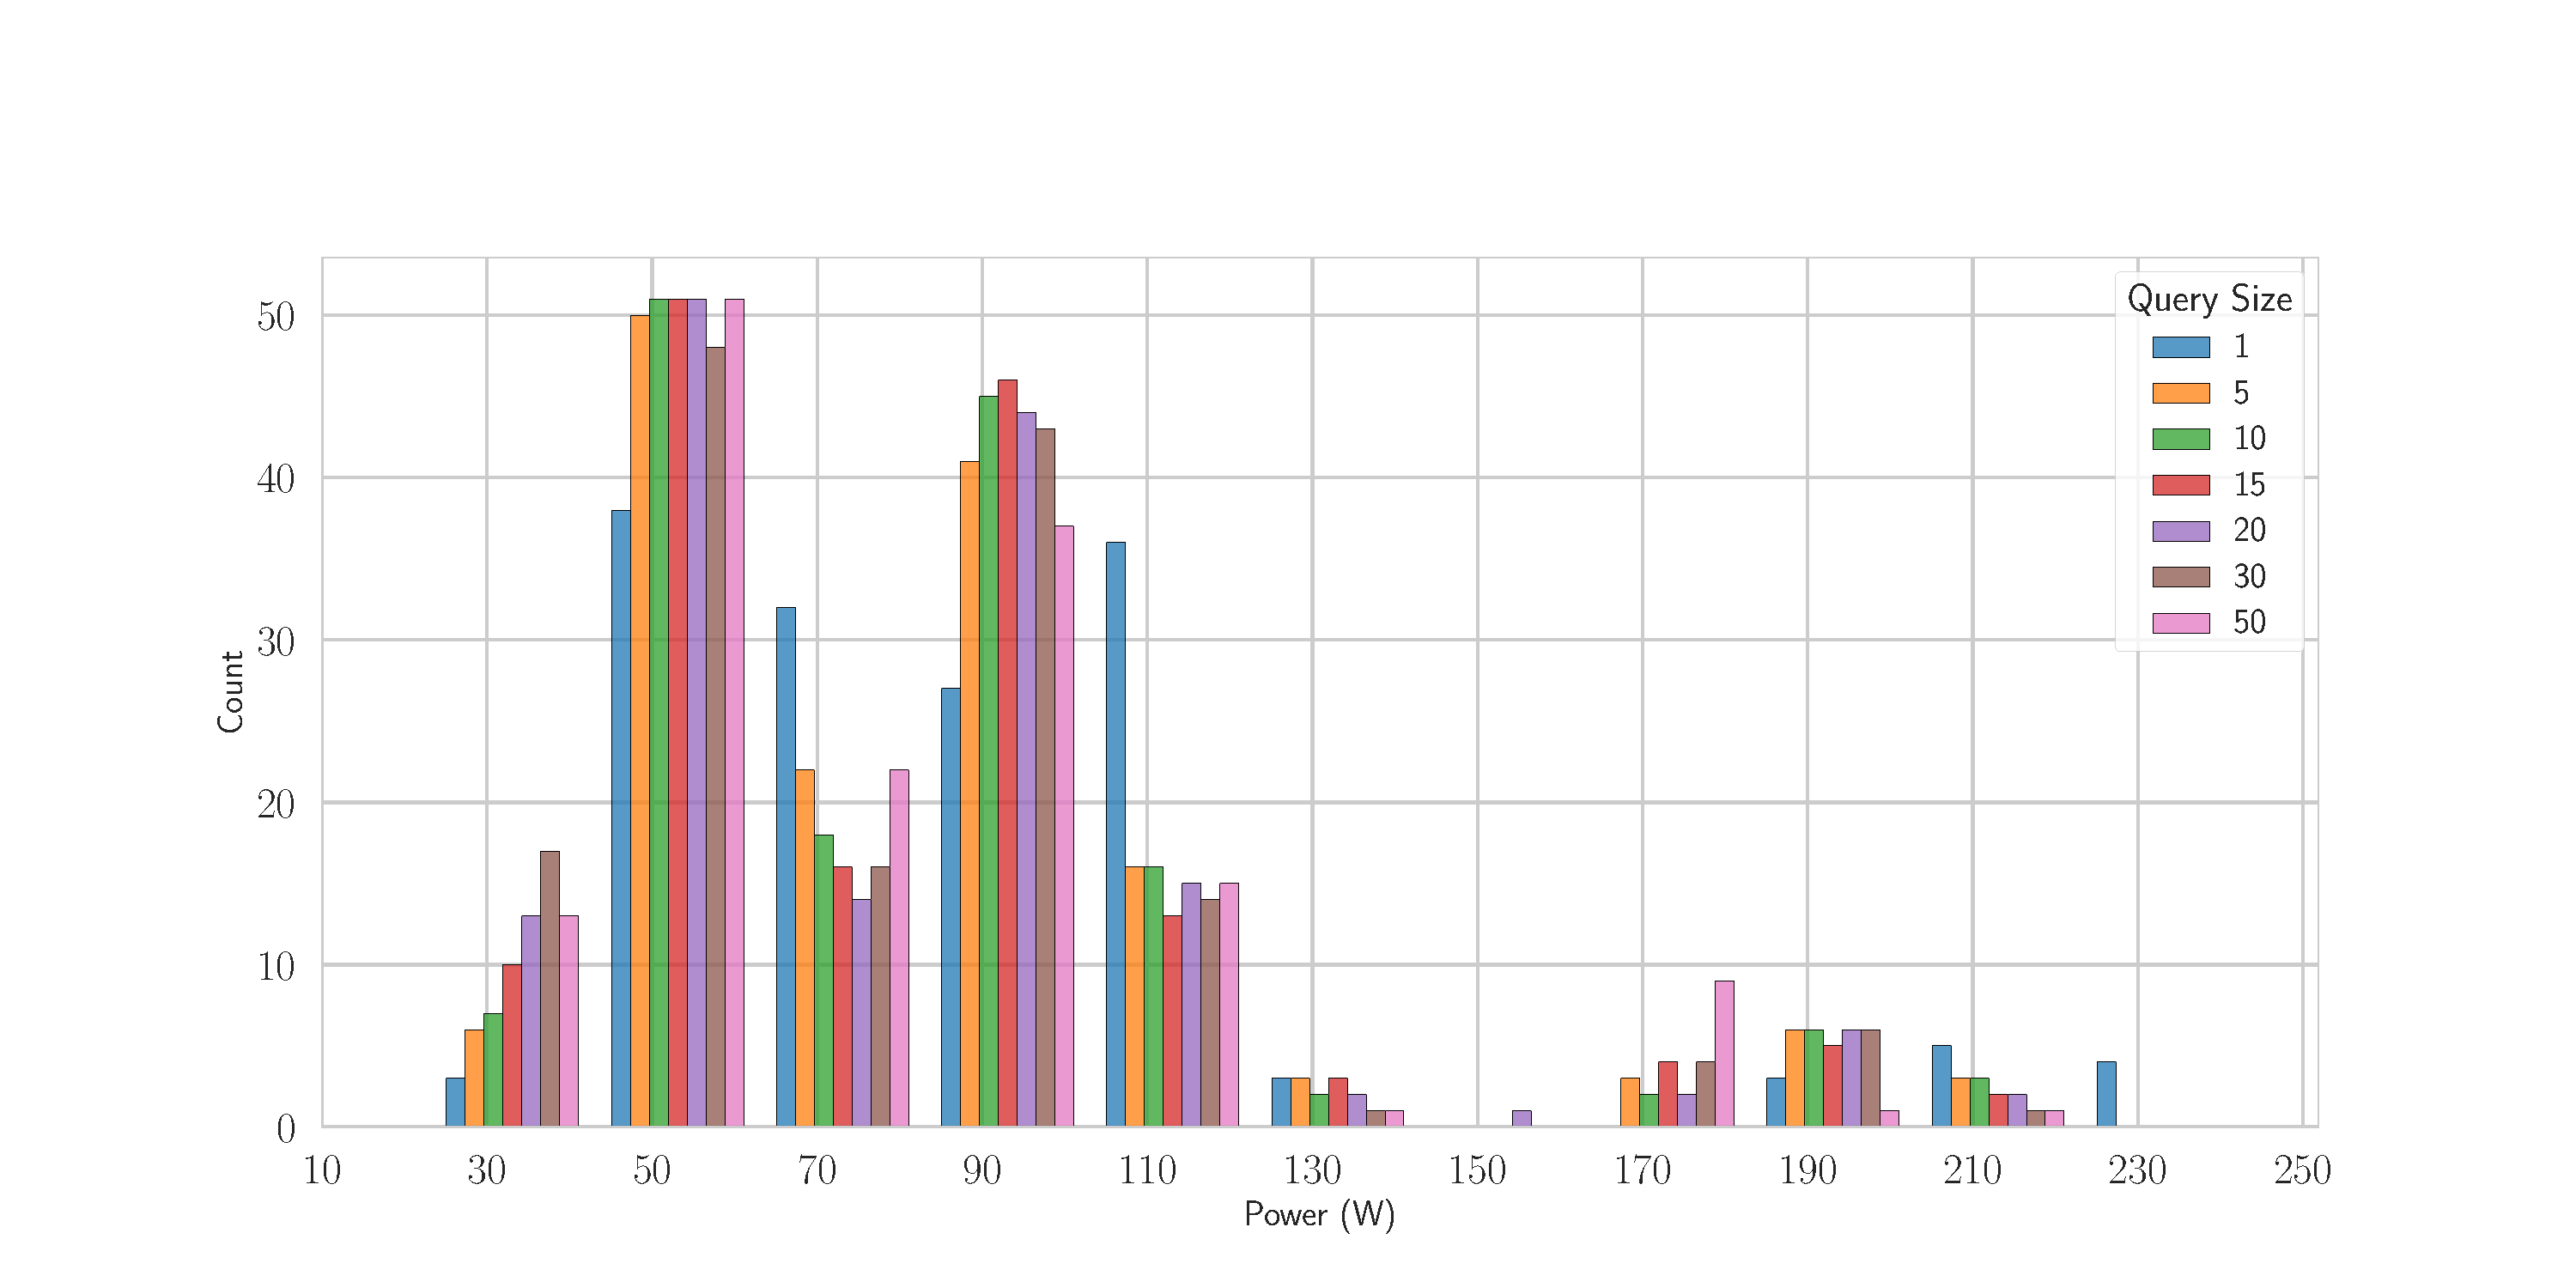
\includegraphics[width=\textwidth,height=\textheight,keepaspectratio]{imgs/histogram_av_power_cpu_update}
    \caption{Average power consumption for the update benchmark}
    \label{fig:av_power_update}
\end{figure}

Figure~\ref{fig:power_requests_update} reports on the number of RPS per level for each framework.
Swoole dropped in the term of performance, while reducing the average power unlike compiled languages based framework, such as lithium and actise.net gained in term of performances while keeping the same power consumption.
Another interesting observation is the linearity between the drop in performance when it comes to requests that contains more than 10 rows.
This drop comes with a slight decrease in average power.

\begin{figure}[hbt]
    % \centering
    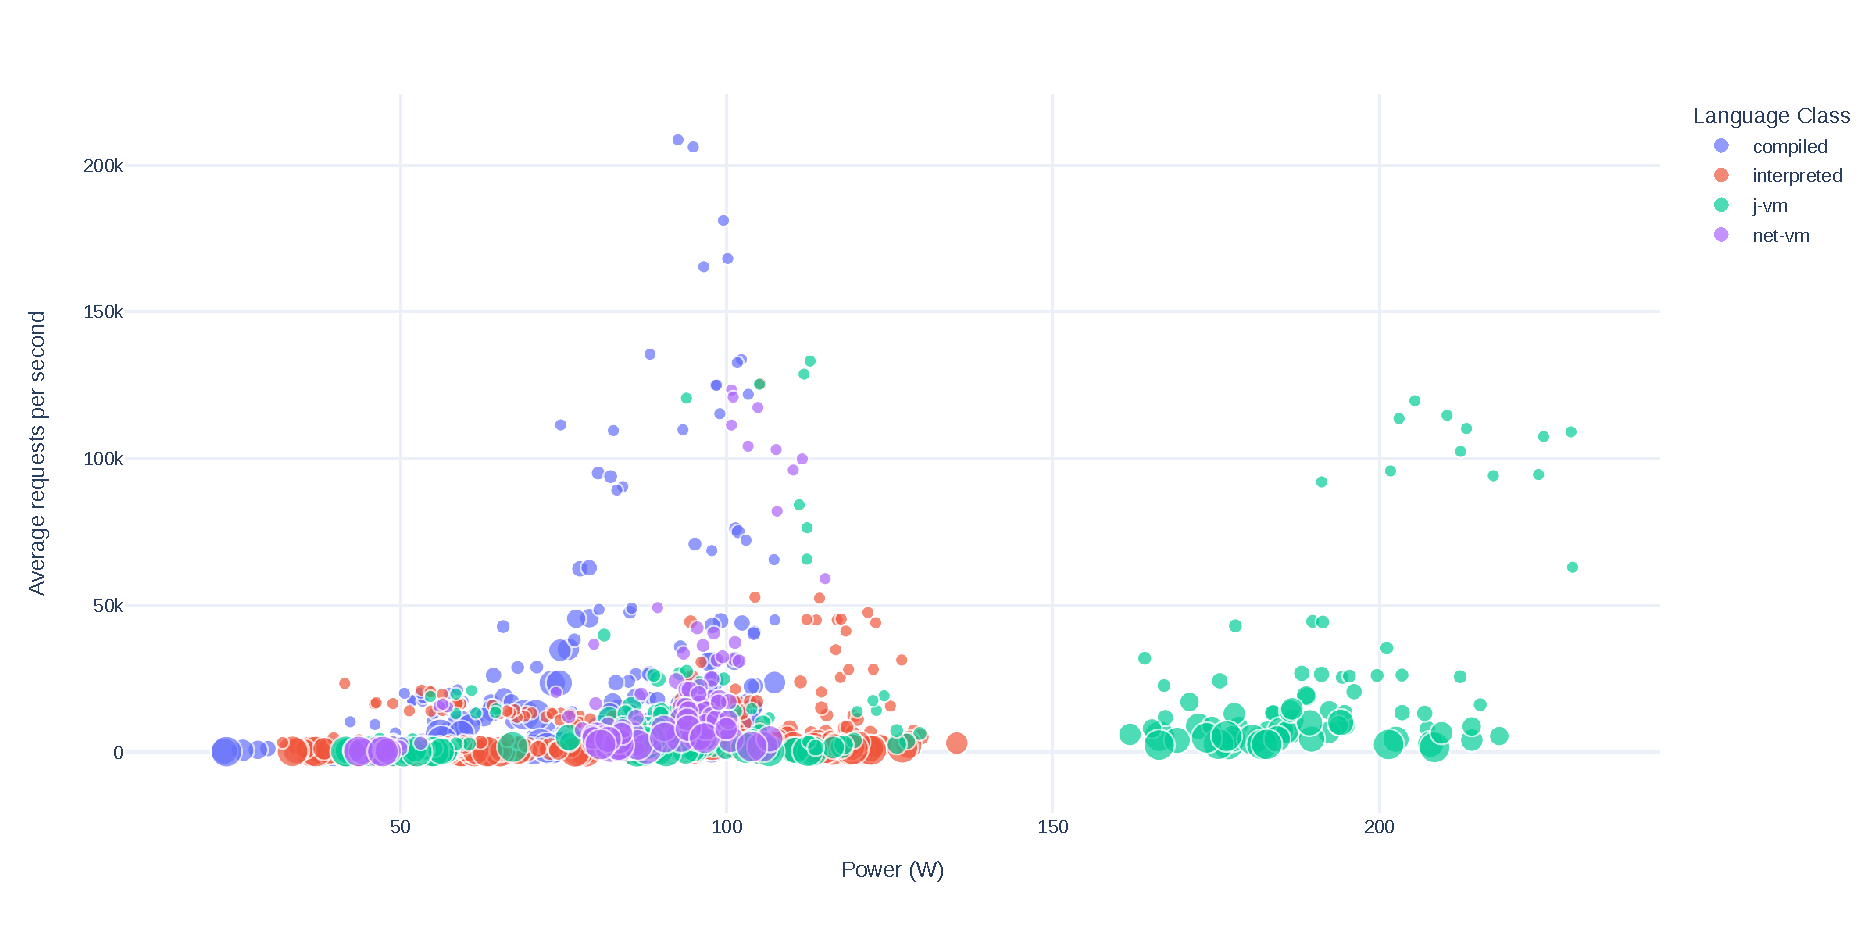
\includegraphics[height=\textwidth,width=\textheight,keepaspectratio,angle=90]{imgs/power_requests_update}
    \caption{Total request Vs average power consumption for the Update benchmark (size of circles represents the number of clients)}
    \label{fig:power_requests_update}
\end{figure}

\paragraph{Plain Text and Json Serialization}
In this scenario, the client hits its limit before servers, as highlighted in Figures~\ref{fig:power_requests_plaintext},\ref{fig:power_requests_json}.
The ceiling is almost linear for the compiled frameworks and the JVM-based ones.
This is also explained by the fact that the high level of stress is on the top, unlike other scenarios.

\begin{figure}[hbt]
    \centering
    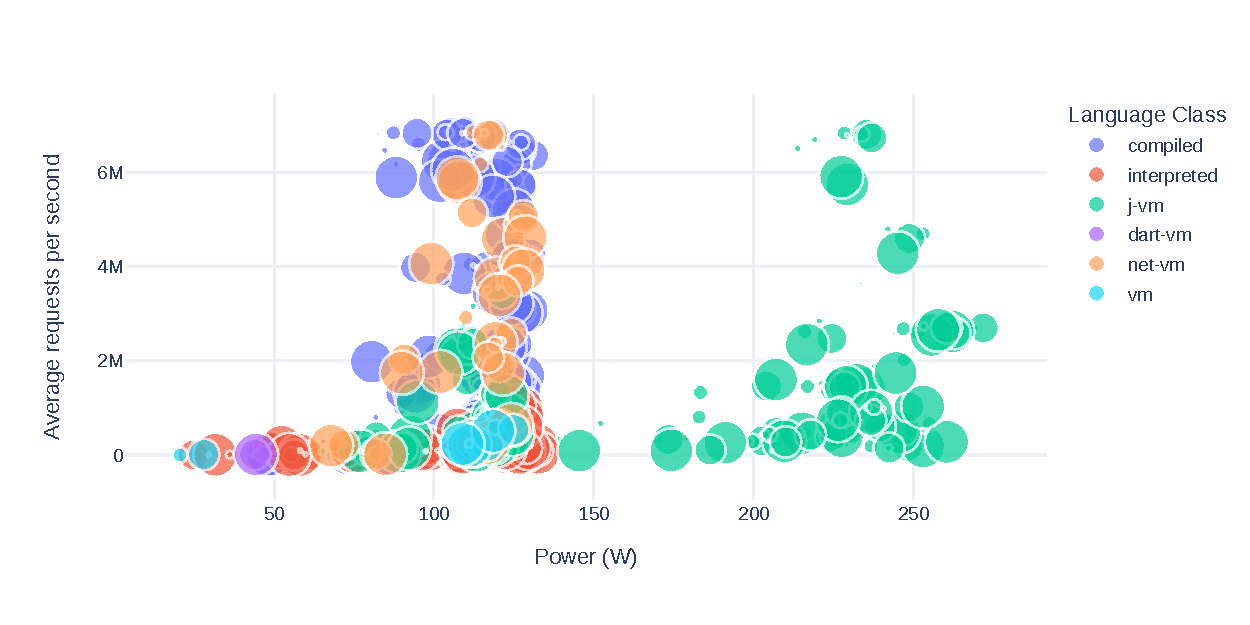
\includegraphics[width=\textwidth,height=\textheight,keepaspectratio]{imgs/power_requests_plaintext}
    \caption{Total request Vs average power consumption for plainText benchmark (size of circles represents the number of clients)}
    \label{fig:power_requests_plaintext}
\end{figure}

\begin{figure}[hbt]
    \centering
    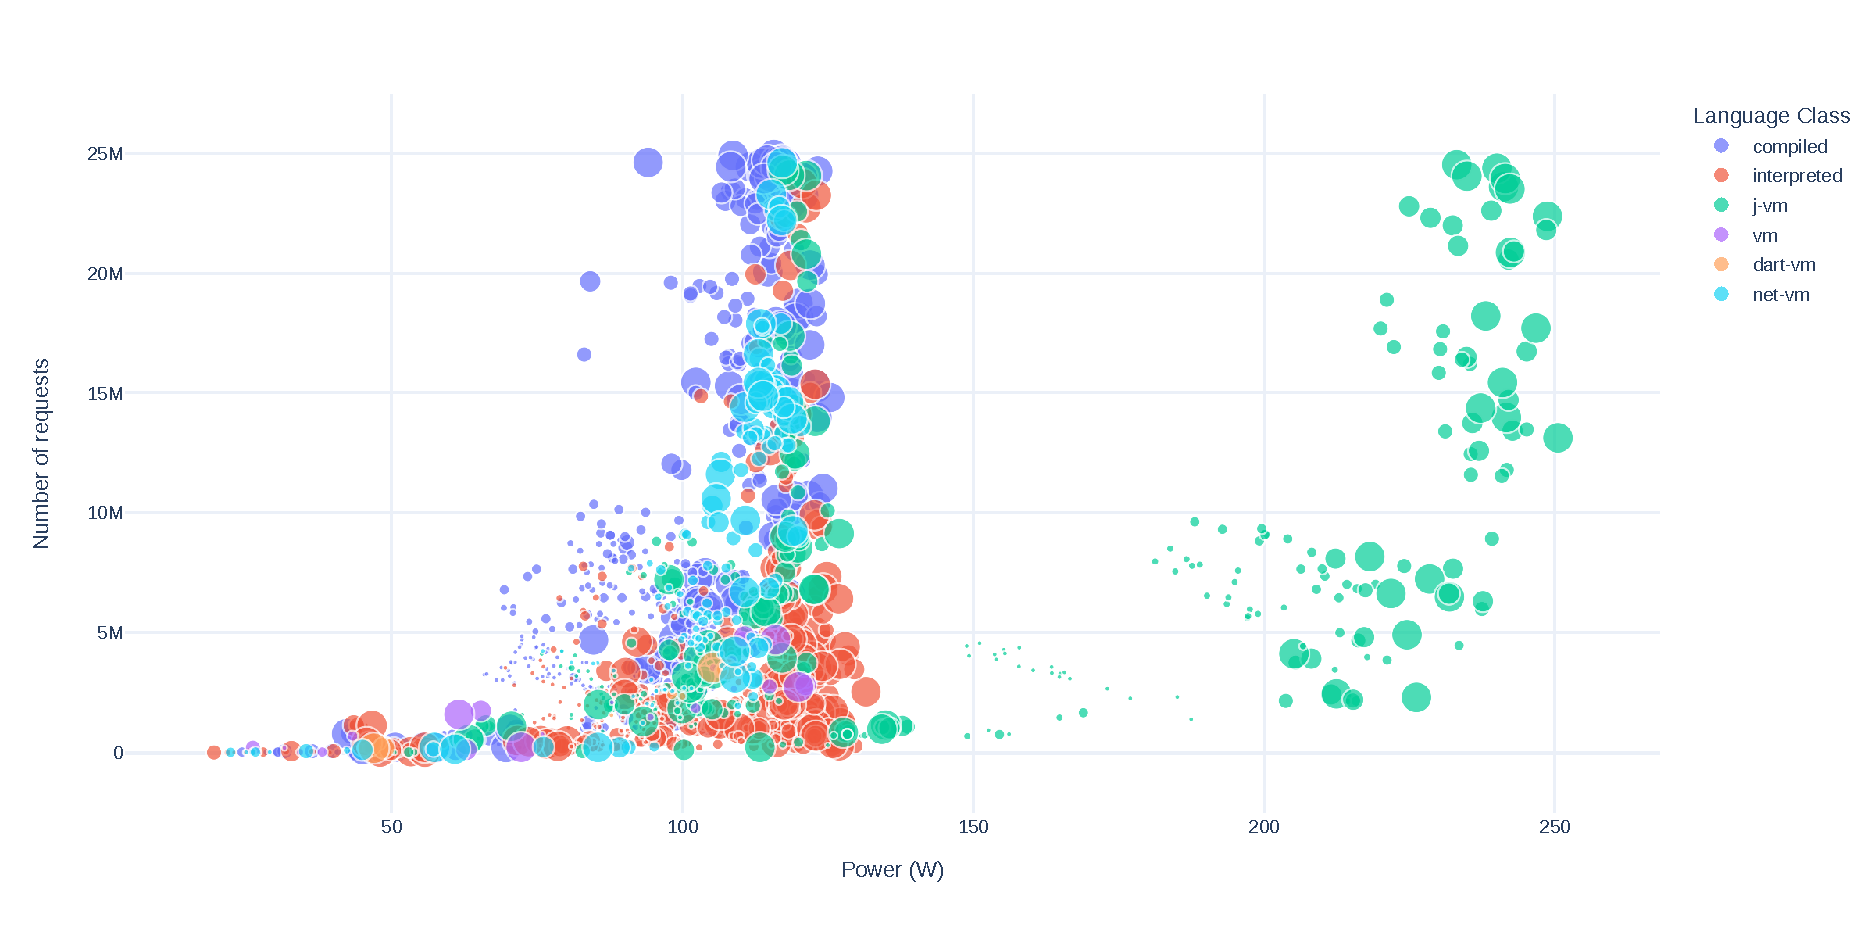
\includegraphics[width=\textwidth,height=\textheight,keepaspectratio]{imgs/power_requests_json}
    \caption{total request vs average power consumption for JSON Serialization test (size of circles represents the number of clients)}
    \label{fig:power_requests_json}
\end{figure}

\subsection{Threats to Validity\note{missing}}
We are aware of the bias inducted by the implementation of a candidates, therefore we propose the framework (see the part of extension) to allow the readers to confirm themselves any new hypothesis.
Regarding a new framework , an new workload a new database ..etc

\subsection{Conclusion\note{missing}}

% \begin{figure}[bht]
%     \centering
%     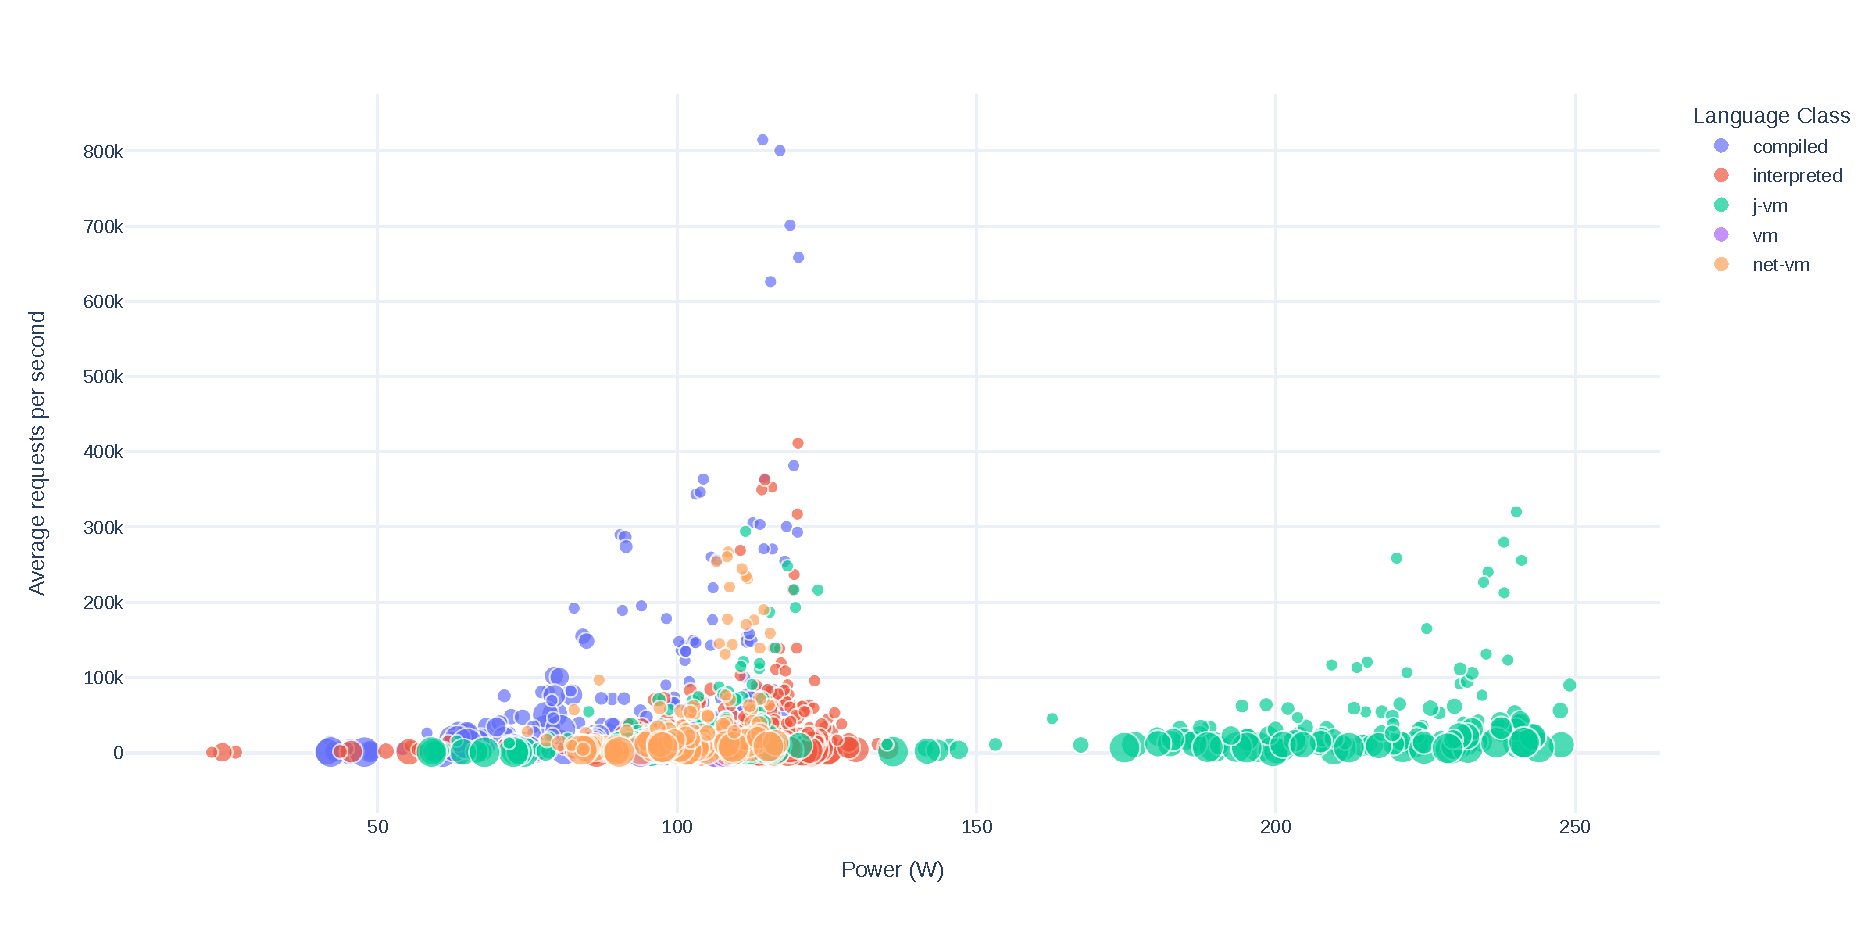
\includegraphics[width=
%         \columnwidth]{imgs/power_requests_query}
%     \caption{total request vs average power consumption for the multiple queries test ( Size of circles represents the size of the query )}
%     \label{fig:power_requests_query}
% \end{figure}
% \begin{figure}[bht]
%     \centering
%     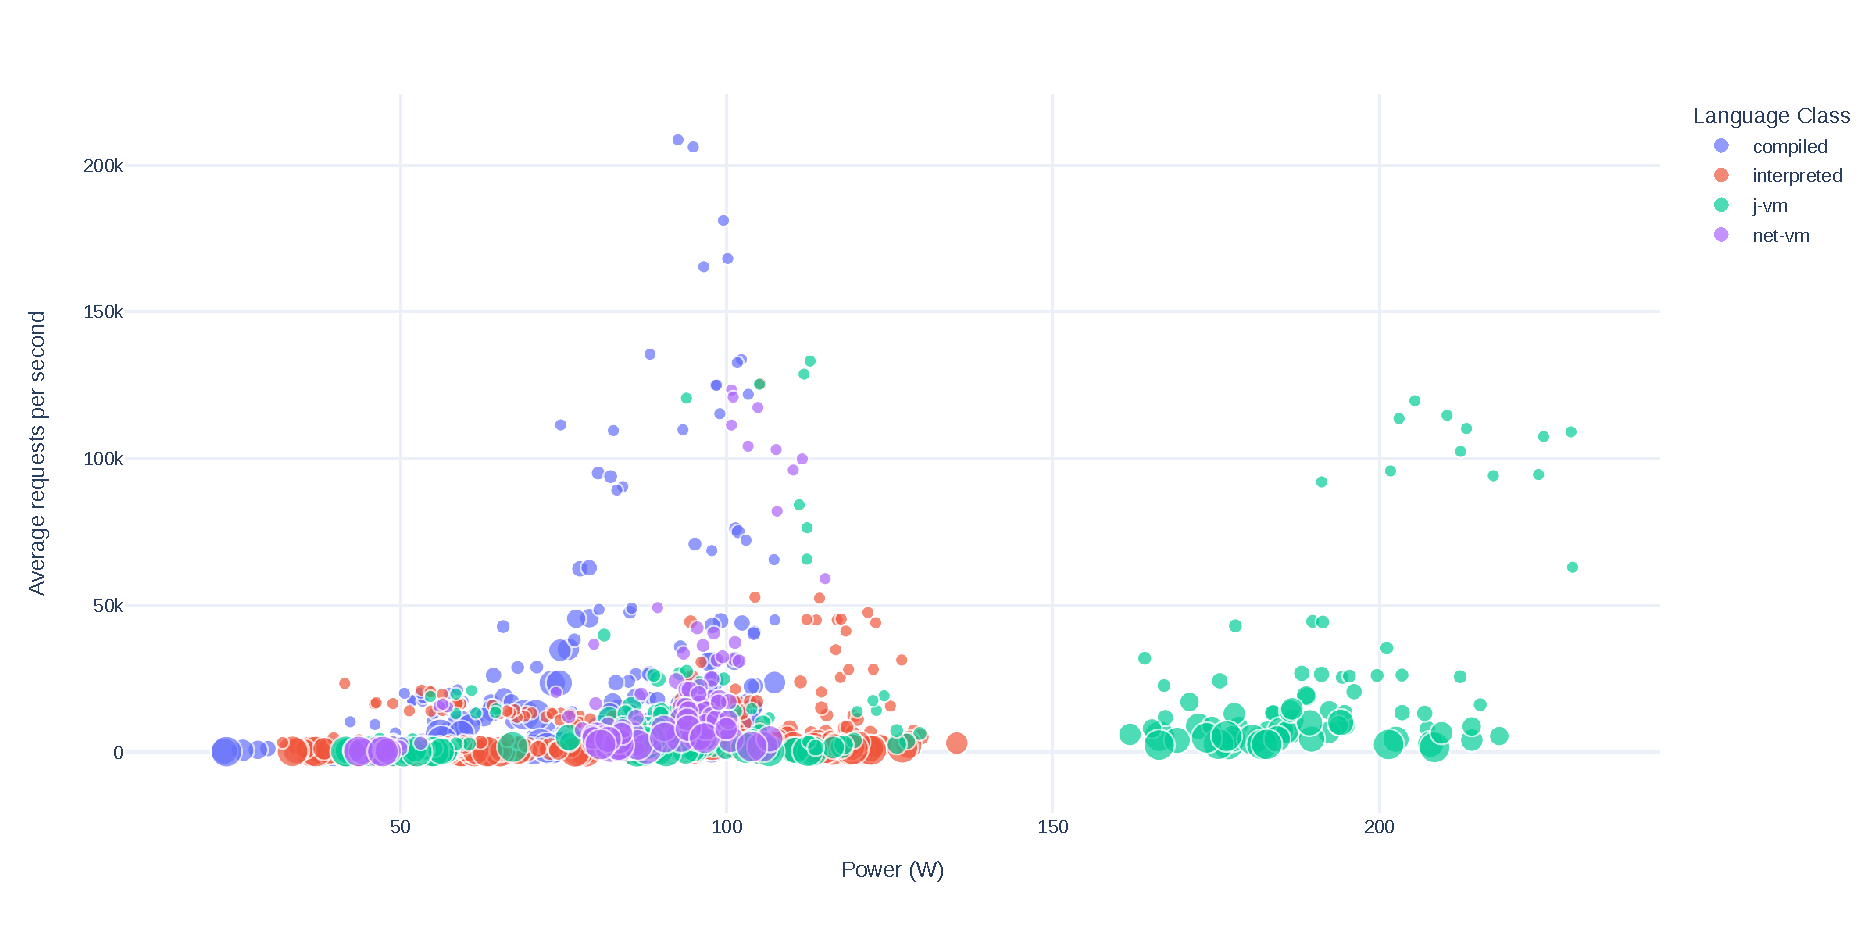
\includegraphics[width=
%         \columnwidth]{imgs/power_requests_update}
%     \caption{total request vs average power consumption for the update queries test ( Size of circles represents the size of the query )}
%     \label{fig:power_requests_update}
% \end{figure}
% \begin{figure}[bht]
%     \centering
%     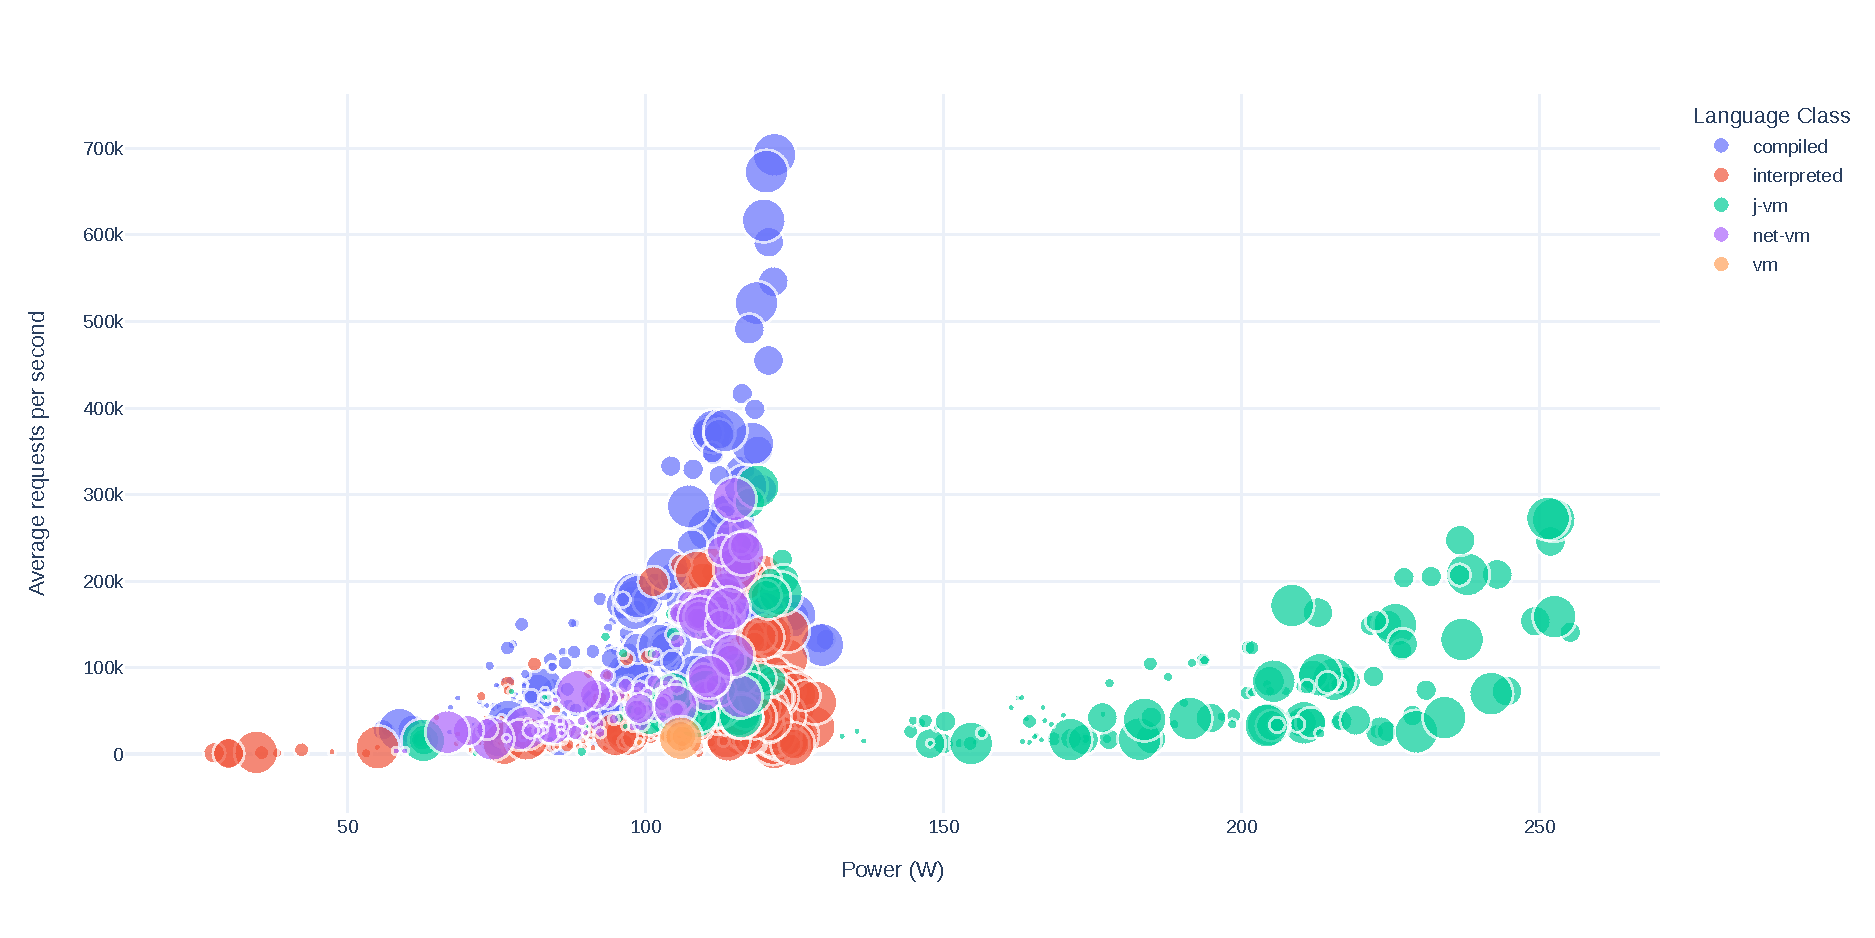
\includegraphics[width=
%         \columnwidth]{imgs/power_requests_fortune}
%     \caption{total request vs average power consumption for Fortunes test ( Size of circles represents the number of clients)}
%     \label{fig:power_requests_fortune}
% \end{figure}
% \begin{figure}[bht]
%     \centering
%     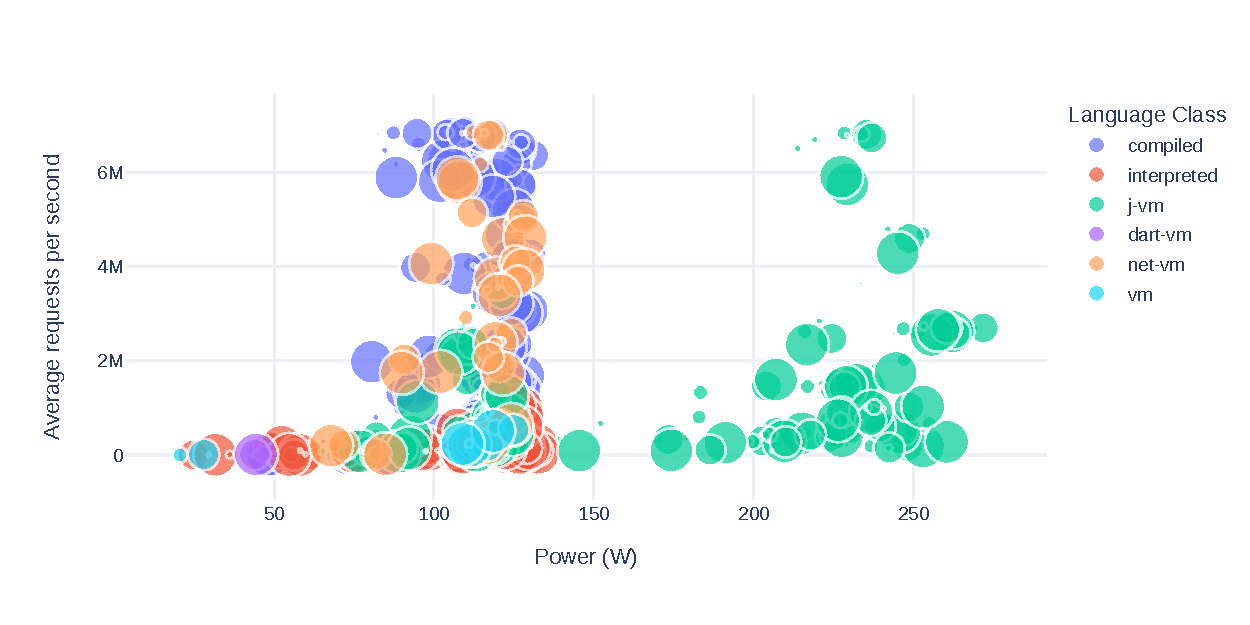
\includegraphics[width=
%         \columnwidth]{imgs/power_requests_plaintext}
%     \caption{total request vs average power consumption for plainText test (size of circles represents the number of clients)}
%     \label{fig:power_requests_plaintext}
% \end{figure}
% \begin{figure}[bht]
%     \centering
%     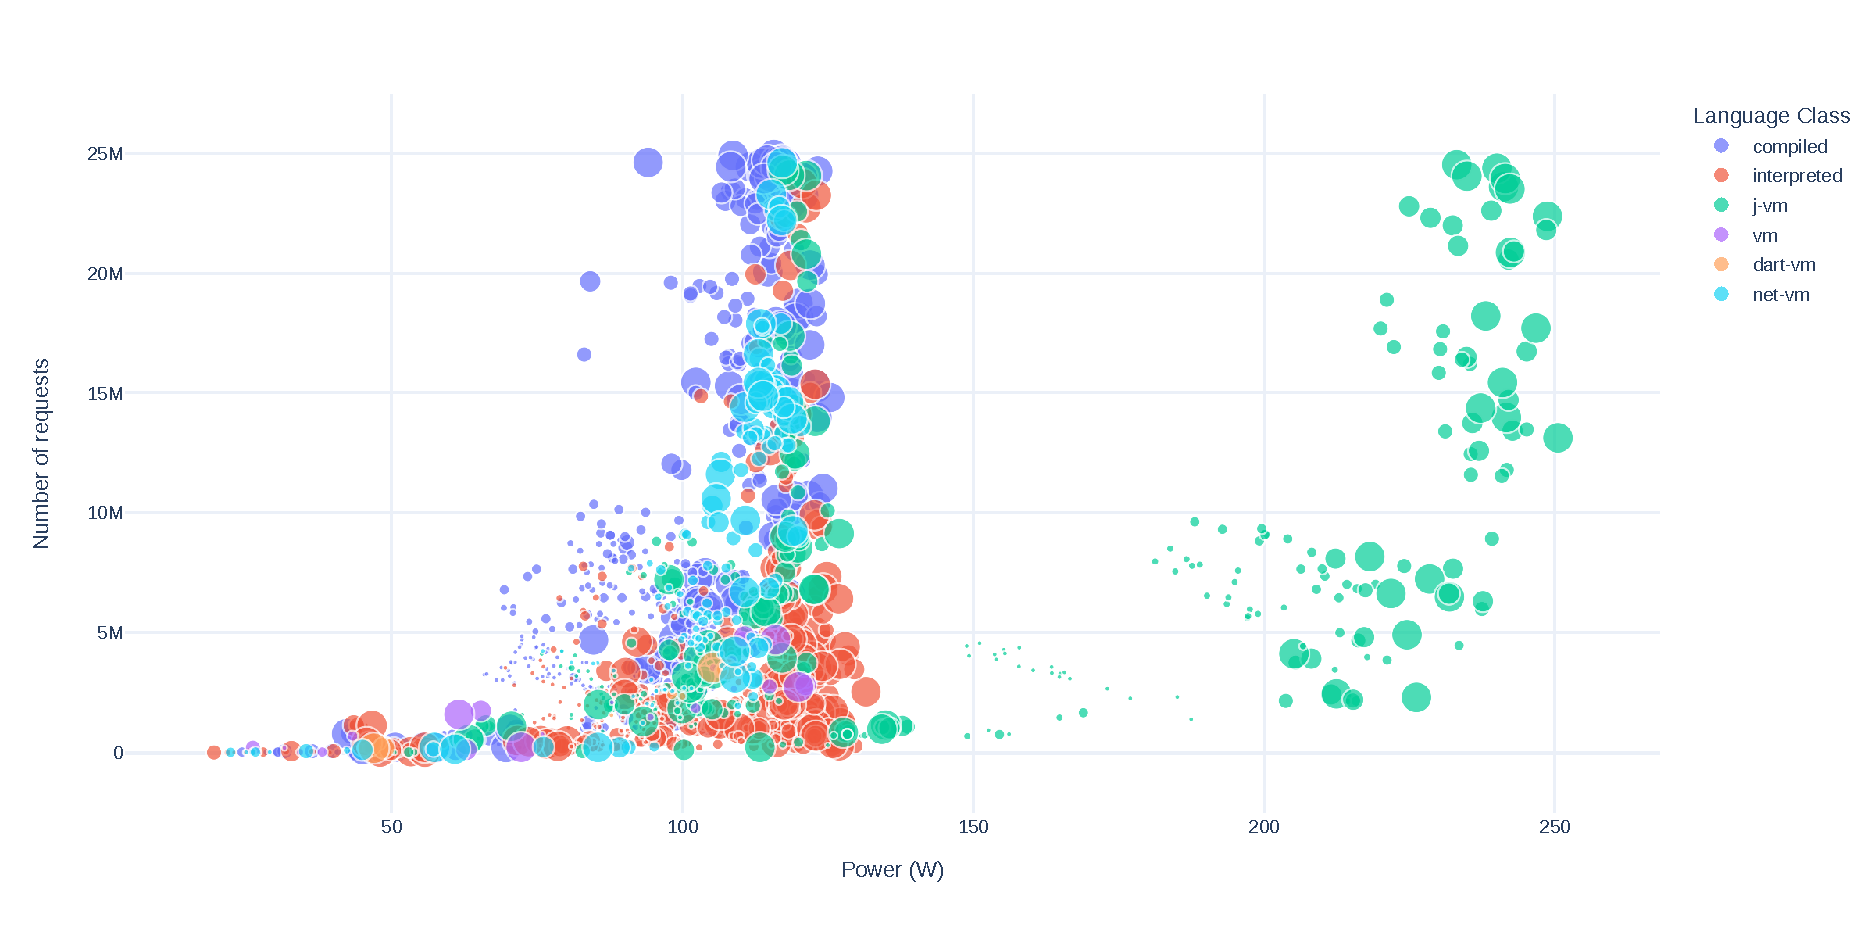
\includegraphics[width=
%         \columnwidth]{imgs/power_requests_json}
%     \caption{total request vs average power consumption for JSON Serialization test (size of circles represents the number of clients)}
%     \label{fig:power_requests_json}
% \end{figure}
% to reduce the space of research we will be looking for some correlation 
% same thing for the number of clients , mayebe we gonna consider 3 cases - 0 , low and high 

%  when comparing static vs dynamic programming langauges we exclude the ones that uses reflection aka C# and JAVA

%% for more about the syntax we recommand cheking this website https://learnxinyminutes.com/

% \newpage

% \subsubsection{tools}
% %TODO : add a table with a single scenarios / check the website for the table
